
\setchapterpreamble[ur]{%
\dictum[T.~Plehn~\cite{plehn_defense}]{%
Did you know that in my PhD defence, I didn't answer a single question correctly?}%
\vspace*{2cm}}

%%%%%%%%%%%%%%%%%%%%%%%%%%%%%%%%%%%%%%%%%%%%%%%%%%%%%%%%%%%%
\chapter{Appendices}
%%%%%%%%%%%%%%%%%%%%%%%%%%%%%%%%%%%%%%%%%%%%%%%%%%%%%%%%%%%%

Here we collect various technical details and intermediate results
that are not too interesting on their own, but should be included for
completeness and reproducibility. We begin with a definition of
different EFT bases and provide a dictionary to translate between
them. Appendix~\ref{sec:appendix_models} then contains some additional
details on the models considered in
\autoref{chapter:validity}. Finally, in
Appendix~\ref{sec:appendix_information} we derive some of the key
results of \autoref{chapter:information}.

Large parts of this appendix has been published previously, as part of
the same articles that contained much of the main body of this
thesis. In particular, Appendices~\ref{sec:appendix_bases} and
\ref{sec:appendix_models} was published in
References~\cite{Brehmer:2015rna, Biekotter:2016ecg}, while
Appendix~\ref{sec:appendix_information} contains material published in
Reference~\cite{Brehmer:2016nyr}.



%%%%%%%%%%%%%%%%%%%%%%%%%%%%%%%%%%%%%%%%%%%%%%%%%%%%%%%%%%%%
\section{Effective field theory conventions}
\label{sec:appendix_bases}
%%%%%%%%%%%%%%%%%%%%%%%%%%%%%%%%%%%%%%%%%%%%%%%%%%%%%%%%%%%%

%%%%%%%%%%%%%%%%%%%%%%%%%%%%%%%%%%%%%%%%%%%%%%%%%%%%%%%%%%%%
\subsection{Standard Model setup}
\label{sec:appendix_bases_sm}
%%%%%%%%%%%%%%%%%%%%%%%%%%%%%%%%%%%%%%%%%%%%%%%%%%%%%%%%%%%%

We begin with our conventions for the Standard Model, which also apply to all models of new physics. We parametrise the SM Lagrangian as
%
\begin{multline}
  \lgr{SM}
  \supset
    - \frac 1 4 G^a_{\mu\nu} G^{a\,\mu\nu} - \frac 1 4 W^a_{\mu\nu} W^{a\,\mu \nu} - \frac 1 4 B_{\mu\nu} B^{\mu \nu}
    + \sum_f \overbar f \im \slashed D f
    + (D^\mu \phi)^\dagger (D_\mu \phi) \\
  %
  \phantom{=} \quad - \mu^2 \phisq - \lambda (\phisq)^2
            - \sum_{\text{generations}} \left(    y_u {\twovec {\overbar u} {\overbar d}}_L \tilde \phi \, u_{R} 
                                                           + y_d {\twovec {\overbar u} {\overbar d}}_L \phi \, d_{R}
                                                           + y_\ell {\twovec {\overbar \nu} {\overbar \ell^-}}_L \phi \, \ell_{R}  + \hc  \right )
\end{multline}
%
with covariant derivatives
%
\begin{align}
  D_\mu \phi &= \left( \partial_\mu - \im g \frac {\sigma^a} 2 W^a_\mu - \im \frac {g'} 2 B_\mu \right) \phi
\end{align}



%%%%%%%%%%%%%%%%%%%%%%%%%%%%%%%%%%%%%%%%%%%%%%%%%%%%%%%%%%%%
\subsection{HISZ basis}
\label{sec:appendix_bases_hisz}
%%%%%%%%%%%%%%%%%%%%%%%%%%%%%%%%%%%%%%%%%%%%%%%%%%%%%%%%%%%%

\begin{table}
\begin{tabular}{lll} 
  \toprule
  \multicolumn{3}{c}{HISZ basis} \\
  \midrule
  $\ope{\phi1} = (D_\mu\phi)^\dagger \, (\phi\,\phi^\dagger) \, (D^\mu\phi)$  &
  $\ope{\phi2} = \dfrac{1}{2}\partial^\mu(\phi^\dagger\phi)\,\partial_\mu(\phi^\dagger\phi)$ &
  $\ope{\phi3} = \dfrac{1}{3}(\phisq)^3$ \\[4mm]
  $\ope{GG} = (\phisq)\,G^A_{\mu\nu}\,G^{\mu\nu\, A}$ \\[2mm]
  $\ope{BB} = -\dfrac{g'^2}{4}(\phisq)\,B_{\mu\nu}\,B^{\mu\nu}$ &
  $\ope{WW} = -\dfrac{g^2}{4}(\phisq)\,W^k_{\mu\nu}\,W^{\mu\nu\, k}$ &
  $\ope{BW} = -\dfrac{g\,g'}{4}(\phi^\dagger\sigma^k\phi)\,B_{\mu\nu}\,W^{\mu\nu\, k}$ \\[4mm]
  $\ope{B}  = \dfrac{ig}{2}(D^\mu\phi^\dagger)(D^\nu\phi)\,B_{\mu\nu}$ &
  $\ope{W} = \dfrac{ig}{2}(D^\mu\phi^\dagger)\sigma^k( D^\nu\phi)\,W_{\mu\nu}^k$ \\[2mm]
  \bottomrule
\end{tabular}
\caption{Bosonic CP-conserving Higgs operators in the HISZ basis.}
\label{tab:validity_operators}
\end{table}


%%%%%%%%%%%%%%%%%%%%%%%%%%%%%%%%%%%%%%%%%%%%%%%%%%%%%%%%%%%%
\subsection{SILH basis}
\label{sec:appendix_bases_silh}
%%%%%%%%%%%%%%%%%%%%%%%%%%%%%%%%%%%%%%%%%%%%%%%%%%%%%%%%%%%%

The SILH Lagrangian reads
%
\begin{align}
  \label{eq:EFT} \lgr{EFT} =& \lgr{SM} + \frac{\bar{c}_H}{2v^2}
\, \partial^\mu (\phisq) \, \partial_\mu (\phisq) +
\frac{\bar{c}_T}{2v^2} \, (\phi^\dagger \, \overleftrightarrow{D}^\mu
\, \phi) \, (\phi^\dagger \, \overleftrightarrow{D}_\mu \, \phi)
-\frac{\bar{c}_6\lambda}{v^2} (\phisq)^3 \notag \\ &+
\frac{ig\bar{c}_W}{2m^2_W} \, (\phi^\dagger \, \sigma^k
\overleftrightarrow{D}^\mu\phi) \, D^\nu \, {W^k}_{\mu\nu} +
\frac{ig'\bar{c}_B}{2m_W^2} \, (\phi^\dagger \,
\overleftrightarrow{D}^\mu \, \phi) \, \partial^\nu \, B_{\mu\nu}
\notag \\ &+ \frac{ig \, \bar{c}_{HW}}{m_W^2} \, (D^\mu \,
\phi^\dagger) \, \sigma^k \, (D^\nu \, \phi) \, W^k_{\mu\nu} +
\frac{ig'\bar{c}_{HB}}{m_W^2} (D^\mu\phi^\dagger) \, (D^\nu \, \phi)
\, B_{\mu\nu}\notag \\ &+ \frac{g'^2 \bar{c}_\gamma}{m_W^2} \,
(\phisq) \, B_{\mu\nu} \, B^{\mu\nu} + \frac{g_s^2 \bar{c}_g}{m_W^2}
\, (\phisq) \, G^A_{\mu\nu} \, G^{\mu\nu\, A} \notag \\ &- \left[
\frac{\bar{c}_u}{v^2} \, y_u \, (\phisq) (\phi^\dagger\cdot \,
\overline{Q}_L) \, u_R + \frac{\bar{c}_d}{v^2} \, y_d \, (\phisq)
(\phi \, \overline{Q}_L) \, d_R + \frac{\bar{c}_\ell}{v^2} \, y_\ell
\, (\phisq) (\phi \, \overline{L}_L) \, \ell_R + \text{h.c.} \,
\right] \,.
\end{align}
%
Here, $g = e/{s_w}, g' = e/{c_w}$, and $g_s$ stand for the SM gauge
couplings and $\lambda$ denotes the usual Higgs quartic coupling. The
normalization of the dimension-6 Wilson coefficients $\overline{c}_i$
includes conventional prefactors which reflect a bias concerning their
origin. We present further details on the EFT setup, the translation
between the different bases, and the connection to Higgs observables
in Appendix~\ref{sec:validity_ap-eft}.

%%%%%%%%%%%%%%%%%%%%%%%%%%%%%%%%%%%%%%%%%%%%%%%%%%%%%%%%%%%%



As mentioned in Sec.~\ref{sec:theory_eff}, we here adopt the notation
and conventions of Reference~\cite{Alloul:2013naa}, which is based on the
SILH framework with the decomposition and
normalization of the Wilson coefficients defined in
Reference~\cite{silh}. For our purposes, it is enough to single
out the subset that encodes all possible new physics contributions to
the Higgs sector compatible with CP conservation and the flavor
structure of the SM. These are given in Tab.~\ref{tab:operators} and
correspond to the Lagrangian in \autoref{eq:EFT}.
 
% \begin{table}
%     \renewcommand{\arraystretch}{1.3}
%     \begin{tabular}[t]{r @{${}={}$}l} 
%       \toprule
%       \multicolumn{2}{c}{Higgs fields}  \\
%       \midrule
%       $\ope{H}$ & $\partial^\mu(\phi^\dagger\,\phi)\,\partial_\mu\,(\phi^\dagger\,\phi)$ \\ 
%       $\ope{6}$ & $(\phisq)^3$  \\
%       $\ope{T}$ & $(\phi^\dagger\,\overleftrightarrow{D}^\mu\,\phi)\,(\phi^\dagger\,\overleftrightarrow{D}_\mu\,\phi)$ \\
%       \bottomrule
%       \toprule
%       \multicolumn{2}{c}{Higgs and fermion fields} \\
%       \midrule
%       $\ope{u}$ & $(\phisq)\,(\phi^\dagger\cdot\,\overline{Q}_L)\,u_R$ \\
%       $\ope{d}$ & $(\phisq)\,(\phi\, \overline{Q}_L)\,d_R$ \\
%       $\ope{\ell}$ & $(\phisq)\,(\phi\, \overline{L}_L)\,l_R$ \\
%       \bottomrule 
%     \end{tabular}
%     \hspace*{1cm}
%     \begin{tabular}[t]{r @{${}={}$}l} 
%       \toprule
%       \multicolumn{2}{c}{Higgs and gauge boson fields} \\
%       \midrule
%       $\ope{HB}$ & $(D^\mu\phi^\dagger)\,(D^\nu\phi)\,B_{\mu\nu}$ \\
%       $\ope{HW}$ & $(D^\mu\phi^\dagger)\,\sigma^k\,(D^\nu\,\phi)\,W^k_{\mu\nu}$ \\ 
%       $\ope{g}$ & $(\phisq)\,G^A_{\mu\nu}\,G^{\mu\nu\, A}$ \\
%       $\ope{\gamma}$ & $(\phisq)\,B_{\mu\nu}\,B^{\mu\nu}$ \\
%       $\ope{B}$ & $(\phi^\dagger\,\overleftrightarrow{D}^\mu\,\phi)\,(\partial^\nu\,B_{\mu\nu})$ \\ 
%       $\ope{W}$ & $\left(\phi^\dagger\,\sigma^k\,\overleftrightarrow{D}^\mu\phi\right)\,(D^\nu\,W^k_{\mu\nu})$ \\
%       \bottomrule
%     \end{tabular}
%   \caption{Dimension-6 operators considered in our analysis. These
%     correspond to a subset of the most general effective operator basis
%     ~\cite{silh} describing new physics effects to the SM
%     Higgs sector with CP-invariance and SM-like fermion structures.}
%   \label{tab:operators}
% \end{table}

The conventions for how covariant derivatives act on the Higgs,
fermion and gauge vector fields are fixed as follows:
%
\begin{align}
  D_\mu \phi &= \partial_\mu \phi - \dfrac {i g'} 2 B_\mu \phi - i g \dfrac {\sigma^a} 2 \, W^a_\mu \, \phi \,,\notag \\
  D_\mu F_L &= \partial_\mu F_L - i g' \dfrac{Y_{F_L}} 2 B_\mu F_L - i g \dfrac {\sigma^a} 2 \, W^a_\mu \, F_L \,,\notag \\
  D_\mu V_\nu^a &= \partial_\mu V_\nu^a + g \, \varepsilon^{abc} \, W_\mu^b \, V_\nu^c \,,\notag \\
  D_\mu W^a_{\nu \rho} &= \partial_\mu W_{\nu \rho}^a + g \, \varepsilon^{abc} \,W_\mu^b \, W_{\nu\rho}^c \,. 
\label{eq:covariant}
\end{align}
%
While the effective Lagrangian in \autoref{eq:EFT} is written in
terms of the fundamental SM gauge fields, the connection to physics
observables is more easily seen in the mass-eigenstate basis, which we
can write as
%
\begin{alignat}{5}
 \lgr{} \supset & -\dfrac{m^2_{H}}{2v}\,g^{(1)}_{HHH}\,HHH  + \dfrac{1}{2}\,g_{HHH}^{(2)}\,H(\partial_\mu H)\,(\partial^\mu H) \notag \\
  & - \dfrac{1}{4}\,g_{ggH}\,G^{\mu\nu\,A}\,G_{\mu\nu}^A\,H - \dfrac{1}{4}\,g_{\gamma\gamma H}\,F^{\mu\nu}\,F_{\mu\nu}\,H \notag \\
  & -\dfrac{1}{4}\,g_{Z}^{(1)}\,Z_{\mu\nu}\,Z^{\mu\nu}\,H -g_{Z}^{(2)}\,Z_{\nu}\,\partial_\mu \,Z^{\mu\nu}\,H + \dfrac{1}{2}\,g^{(3)}_{Z}\,Z_\mu Z^{\mu}\,H \notag 
  \\
  & - \dfrac{1}{2}\,g_{W}^{(1)}\,W^{\mu\nu}\,W^\dagger_{\mu\nu}\,H - 
  \left[g_{W}^{(2)} W^\nu\,\partial^\mu W^\dagger_{\mu\nu} H + \text{h.c.} \right] + g_{W}^{(3)}\,m_W\,W^\dagger_\mu W^\mu\, H \notag \\ 
  & -\left[g_{u}\dfrac{1}{\sqrt{2}}\left(\bar{u}P_R u\right)H + g_{d}\dfrac{1}{\sqrt{2}}\left(\bar{d}P_R d\right)H + g_{\ell}\dfrac{1}{\sqrt{2}}\left(\bar{\ell}P_R \ell\right)H + \text{h.c.}
  \right]
 \label{eq:masslag},
\end{alignat}
%
with the different effective couplings $g_i$ quoted in
Tab.~\ref{tab:coefficients}.  More details on the notation and
conventions can be found in Reference~\cite{Alloul:2013naa}.

\begin{table}
  \renewcommand{\arraystretch}{1.2}
  \begin{tabular}{r l l}
    \toprule
    Coupling & Operators & Expression \\
    \midrule
    $g^{(1)}_{Z} $ & $\ope{HB}, \ope{HW}, \ope{H}gam$ & $\frac{2g}{m_Wc^2_w}\left[\bar{c}_{HB}s^2_w-4\bar{c}_{\gamma}s_w^4+c^2_w \,\bar{c}_{HW} \right] $ \\
    $g^{(2)}_{Z} $ & $\ope{HW}, \ope{HB}, \ope{W}, \ope{B}$ & $ \frac{g}{m_Wc^2_w}\left[(\bar{c}_{HW} + \bar{c}_W)c^2_w + (\bar{c}_B + \bar{c}_{HB})s^2_w\right]$\\  
    $g^{(3)}_{Z} $ & $\ope{H}, \ope{T}, \ope{\gamma}$ & $\frac{g m_W}{c_w^2}\left[1-\frac{1}{2}\bar{c}_H - 2\bar{c}_T + 8\bar{c}_\gamma\frac{s_w^4}{c^2_w} \right]$ \\
    \midrule
    $g^{(1)}_{W} 
    $ & $\ope{HW}$ & $\frac{2g}{m_W}\,\bar{c}_{HW} $ \\
    $g^{(2)}_{W}$ & $\ope{HW},\ope{W}$ & $\frac{g}{m_W}\,\left[\bar{c}_W + \bar{c}_{HW}\right]$ \\  
    $g^{(3)}_{W}$ & $\ope{H}$ & $g(1-\frac{1}{2}\bar{c}_H)$\\
    \midrule
    $g_{f}$ & $\ope{H}, \ope{f} \quad (f = u,d,\ell)$ & $\frac{\sqrt{2}m_f}{v}\left[1-\frac{1}{2}\bar{c}_H + \bar{c}_f\right] $ \\
    \midrule
    $g_{g} $ & $\ope{H}, \ope{g}$ & $g_H - \frac{4 \bar{c}_g g_s^2 v}{m_W^2}$ \\
    \midrule
    $g_{\gamma}$ & $\ope{H}, \ope{\gamma}$ & $a_H - \frac{8 g \bar{c}_\gamma s^2_w}{m_W}$\\
    \midrule
    $g^{(1)}_{HHH}$  & $\ope{H}, \ope{6}$ & $1+\frac{5}{2} \bar{c}_6 - \frac{1}{2}\bar{c}_{H}$ \\ 
    $g^{(2)}_{HHH} $  & $\ope{H}$ & $\frac{g}{m_W}\,\bar{c}_H$ \\
    \bottomrule
  \end{tabular} 
  \caption{Subset of the dimension-6 operators which enter the different
    leading-order Higgs couplings which are relevant for LHC
    phenomenology, in the notation and conventions of
    Reference~\cite{Alloul:2013naa} (see text).  The different superscripts
    denote the various terms in the Lagrangian in \autoref{eq:masslag} and
    correspond to either a SM-like interaction with a rescaled coupling
    strength or to genuinely new Lorentz structures. The weak coupling
    constant is written as $g \equiv e/s_w$.  The SM contribution to the
    loop-induced Higgs coupling to the gluons (photons) is denoted by
    $g_H$ ($a_H$).}
  \label{tab:coefficients}
\end{table}

Note that the Higgs-fermion coupling shift is given by $g_f \propto
y_f (1 - \bar{c}_H/2  +  3 \bar{c}_f/2)$, but $\ope{f}$ also
shifts the fermion masses to $m_f = y_f v (1 + \bar{c}_f/2) /
\sqrt{2}$, yielding the result given above. Similarly, $\ope{H}$ and
$\ope{\gamma}$ generate additional contributions to the Higgs-boson and
gauge-boson kinetic terms, which are restored to their canonical form
by the field re-definitions
%
\begin{align}
H &\to H \, \left(1-\dfrac{1}{2}c_H \right), & 
Z_\mu &\to Z_\mu \, \left( 1+\dfrac{4s_w^4}{c_w^2}c_\gamma \right) \,,\notag \\
&& 
A_\mu &\to A_\mu \, \left( 1+4s_w^2 \, c_\gamma \right) -
  Z_\mu \left( \dfrac{8s_w^3}{c_w} c_\gamma \right).
\end{align}
%
None of the operators considered in this basis affects the relations
between $g$, $m_W$, $v$ and $G_F$, so the SM relations
%
\begin{align}
  m_W &= \dfrac {g\,v} 2 \,, &
  G_F &=\dfrac {\sqrt{2} \, g^2} {8\, m_W^2} = \dfrac 1 {\sqrt{2} v^2} \,,
\end{align}
%
can always be used to translate these coupling shifts from one scheme
of input parameters to another.

Dimension-6 operators result in a modified pattern of Higgs
interactions, leading to coupling shifts $g_{xxH} \equiv
g_{xxH}^\text{SM}(1+\Delta_x)$ and also genuinely novel Lorentz
structures. Interestingly, in general more than one of the
effective operators in Tab.~\ref{tab:operators} contributes to a
given Higgs interaction in the mass basis, implying that it is in
general not possible to establish a one-to-one mapping between Wilson
coefficients and distorted Higgs couplings.

Note that the Wilson coefficients of the operators $\ope{T}$ and $\ope{B}+\ope{W}$
are strongly constrained by electroweak precision data~\cite{silh}. In
this work, we allow ourselves, on occasion, to ignore these bounds to
more distinctly illustrate the effects in the Higgs sector.

Translations between effective operator bases can be performed with
the help of equations of motion, field redefinitions, integration by
parts and Fierz identities. Here we quote a number of such relations
which turn out to be particularly useful for the practitioner. For
example, in addition to the effective operators in the SILH basis,
we often find the operators
%
\begin{align}
  \ope{r} &= \phisq\, (D_\mu \phi)^2\,, &
  \ope{HF}' &= \left( \bar{f}_L \, \gamma^\mu \, \sigma^a \, f_L \right) \left( \phi^\dagger \, \sigma^a \, \overleftrightarrow{D}_\mu \, \phi \right)  \,,
  \notag \\
  \ope{D} &= \left( D^2 \, \phi \right)^2\,, &
  \hat{\ope{}}'_{HH} &= \left( \phi^\dagger \, \sigma^a \, \overleftrightarrow{D}_\mu \, \phi \right)\left( \phi^\dagger \, \sigma^a \, \overleftrightarrow{D}_\mu \, \phi \right)\,.
  \label{eq:EFT_OHf}
\end{align}
%
$\hat{\ope{}}'_{HH}$ can be replaced by using the completeness relation of the Pauli matrices, which for arbitrary SU(2) doublets $\xi,\,\chi,\,\eta,\,\psi$ leads to
\begin{align}
(\xi^\dagger \sigma^a \chi)(\eta^\dagger \sigma^a \psi) &=
\sum_{ijkl} \xi^*_i \sigma^a_{ij} \chi_j \, \eta^*_k \sigma^a_{kl} \psi_l \notag \\
&= \sum_{ijkl} (2\delta_{il}\delta_{jk}-\delta_{ij}\delta_{kl})\xi^*_i \chi_j \, \eta^*_k \psi_l = 2(\xi^\dagger\psi)(\eta^\dagger\chi)-(\xi^\dagger \chi)(\eta^\dagger\psi)\,.
\end{align}
Thus we find
\begin{align}
\hat{\ope{}}'_{HH} &= (\phi^\dagger\,\sigma^a\,D^\mu \phi)^2
+((D^\mu\phi^\dagger)\,\sigma^a\,\phi)^2
-2((D^\mu\phi^\dagger)\,\sigma^a\,\phi)(\phi^\dagger\,\sigma^a\,D_\mu \phi) \notag \\
&= (\phi^\dagger\,D^\mu \phi)^2
+ ((D^\mu\phi^\dagger)\,\phi)^2
-2\left[ 2((D^\mu\phi^\dagger)\,D^\mu \phi)(\phi^\dagger\phi) - 
 ((D^\mu\phi^\dagger)\,\phi)(\phi^\dagger\,D^\mu \phi) \right]
\notag \\
&= \ope{H} - 4 \ope{r} \,.
  \label{eq:EFT_JHJH_replacement}
\end{align}
%
The equation of motion for the $W$ fields,
%
\begin{align}
D^\nu W^a_{\mu \nu} 
= - i g \, \phi^\dagger \dfrac {\sigma^a} {2} \overleftrightarrow{D}_\mu \phi 
  - g \sum_f \bar{f}_L \dfrac {\sigma^a} {2} \gamma_\mu f_L  \,,
 \label{eq:eom-w}
\end{align}
gives rise to the identity
\begin{align}
  \sum_f \ope{HF}' = \dfrac {2} {g} \, \ope{W} - {i} \, \ope{H} + 4 i \, \ope{r}  \,.
  \label{eq:EFT_OHf_replacement}
\end{align}
%
A global redefinition $\phi \to \phi + \alpha \, (\phisq) \phi / v^2$ generates a shift in the Wilson coefficients
\begin{alignat}{5}
 c_H \to c_H + 2\alpha\,, \quad
 c_r \to c_r + 2\alpha\,, \quad c_6 \to c_6 {+} 4\alpha\,, \quad c_f \to c_f {+} \alpha\,,
 \label{eq:wilson-shift}
\end{alignat}
so that
with the choice $\alpha=-c_r/2$ one can eliminate the operator
$\ope{r}$ in favor of other operators:
%
\begin{align}
  \ope{r} \leftrightarrow \biggl\{ - \dfrac 1 2 \, \ope{H} + 2 \, \lambda \, \ope{6} + \sum_f \left[ \dfrac 1 2 \, y_f \, \ope{f} + \text{h.c.}\right] \biggr\} \,.
  \label{eq:EFT_Or_replacement}
\end{align}
%
Finally, $\ope{D}$ can be exchanged for others using the equation of motion for
$\phi$,
%
\begin{align}
  D^2 \phi &= - \mu^2  \, \phi - 2\, \lambda \, \phisq \, \phi - \sum_\text{gen.} \left[y_u \, \bar{Q}^T_L \, u_R + y_d \, \bar{d}_R \, Q_L + y_\ell \, \bar{\ell}_R \, L_L \right] \,. 
\end{align}
%
This leads to
%
\begin{align}
  \ope{D} = \mu^4 \, \phisq 
 + 4 \, \lambda \, \mu^2 \, (\phisq)^2 
 + \mu^2 \, \sum_f y_f \, \bar{f}_L \phi f_R  \
 + 4 \, \lambda^2 \, (\phisq)^3 + 2 \, \lambda \, \sum_f y_f \, \phisq \, \left( \bar{f}_L \phi f_R \right) \,.
\end{align}
%
The first three terms lead to a renormalization of the SM parameters
$\mu$, $\lambda$, $y_f$, without any impact on physical
observables. The last two terms, however, means that $\ope{D}$ is
equivalent to the combination
%
\begin{align}
  \ope{D} \leftrightarrow 4 \, \lambda^2 \, \ope{6} + 2 \, \lambda \, \sum_f \left( y_f \, \ope{f} + \text{h.c.} \right)\,.
  \label{eq:EFT_OD_replacement}
\end{align}





%%%%%%%%%%%%%%%%%%%%%%%%%%%%%%%%%%%%%%%%%%%%%%%%%%%%%%%%%%%%
\subsubsection{SILH to HISZ}
%%%%%%%%%%%%%%%%%%%%%%%%%%%%%%%%%%%%%%%%%%%%%%%%%%%%%%%%%%%%

We also give the conversion to the popular HISZ
basis~\cite{Hagiwara:1993ck} (see also
References~\cite{Corbett:2012ja,sfitter_last} for recent studies in
this framework)
%
\begin{align}
  \lgr{HISZ} = \sum_i \dfrac{f_i} {\Lambda^2} \ope{i}' \, ,
\end{align}
%
with Higgs-gauge operators given in Tab.~\ref{tab:ops2}.  We use the
same conventions for the covariant derivative as above (note that this
is not the case in some of the cited literature). The operators can
then be translated via the relations
%
\begin{align}
\ope{H}  &= 2\ope{\phi2}'\,, \qquad &
\ope{W}  &= \dfrac{2 i}{g}  \left( \ope{WW}' +  \ope{BW}' - 2\ope{W}'   \right)\,,  \quad & 
\ope{HW} &= -\dfrac{2i }{g} \ope{W}'\,,  \notag \\ 
\ope{T}  &= 2\ope{\phi2}'  -  4\ope{\phi1}'\,,  &
\ope{B}  &= \dfrac{2 i}{g'}  \left( \ope{BB}' +  \ope{BW}' - 2\ope{B}' \right)\,, & 
\ope{g}  &= \ope{GG}' \,,  \notag \\
\ope{6} &= 3 \ope{\phi3}' \,, & 
\ope{HB}  &= -\dfrac{2 i }{g'}\ope{B}'\,, & 
\ope{\gamma} &= -\dfrac{4}{g'^2}  \ope{BB}'  \,.
\end{align}
%
The HISZ basis also includes the redundant operator $\ope{\phi4}' =
(D_\mu\phi)^\dagger(D^\mu\phi)\,\phi^\dagger\phi$, which can be
removed using \autoref{eq:EFT_Or_replacement}.  For the coefficients,
we find
%
\begin{align}
  \bar{c}_H &= \dfrac{v^2}{\Lambda^2}\,\left(\dfrac{1}{2}f_{\phi1}+f_{\phi2}\right)\,, &
  \bar{c}_W &= -\dfrac{v^2}{\Lambda^2}\,\dfrac{g^2}{4}f_{WW} \notag\,, \\
  \bar{c}_T &= -\dfrac{v^2}{\Lambda^2}\,\dfrac{1}{2}f_{\phi1}\,, & 
  \bar{c}_B &= \dfrac{v^2}{\Lambda^2}\,\dfrac{g^2}{4} (f_{WW}-f_{BW}) \notag\,, \\
  \bar{c}_6 &= -\dfrac{v^2}{\Lambda^2}\,\dfrac{1}{3\lambda}f_{\phi3}\,, &
  \bar{c}_{HW} &= \dfrac{v^2}{\Lambda^2}\,\dfrac{g^2}{8} (f_{W}+2f_{WW}) \notag\,, \\
  \bar{c}_g &= \dfrac{v^2}{\Lambda^2}\,\dfrac{g^2}{4g_s^2}f_{GG}\,, &
  \bar{c}_{HB} &= \dfrac{v^2}{\Lambda^2}\,\dfrac{g^2}{8} (f_{B}+2f_{BW}-2f_{WW}) \notag\,, \\
  \bar{c}_\gamma &= \dfrac{v^2}{\Lambda^2}\,\dfrac{g^2}{16} (f_{BW}-f_{BB}-f_{WW}) \, .
\end{align}





%%%%%%%%%%%%%%%%%%%%%%%%%%%%%%%%%%%%%%%%%%%%%%%%%%%%%%%%%%%%
\subsection{HLM basis}
%%%%%%%%%%%%%%%%%%%%%%%%%%%%%%%%%%%%%%%%%%%%%%%%%%%%%%%%%%%%

Aside from the relatively simple case of the multi-Higgs sector
extensions, we make use of the covariant derivative
expansion~\cite{Gaillard:1985uh,Cheyette:1987qz} to analytically carry out
the matching between the different UV completions to
their corresponding EFT description.  The method has been recently
reappraised in Reference~\cite{Henning:2014wua} and employed in a number of
studies~\cite{heft_limitations,heft_limitations2,Chiang:2015ura,Huo:2015exa}.
By applying this method, the Wilson coefficients are readily obtained
in a different operator basis (henceforth dubbed HLM),
%
\begin{align}
  \lgr{HLM} = \sum_i \dfrac{k_i} {\Lambda^2} \ope{i}''.
\end{align}
%
The HLM operators involving Higgs fields and their interaction with
gauge bosons are listed in Tab.~\ref{tab:ops2}.  In addition, the HLM
basis contains a subset of operators with no direct correspondence to
the bosonic SILH operators, which must be rewritten with the help of
equations of motion and field redefinitions, as we discuss below.

%-----------------------------------------------------------
\begin{table}
  \renewcommand{\arraystretch}{1.2}
  \setlength{\tabcolsep}{1ex}
  \centering
    \begin{tabular}[t]{r @{${}={}$}l} 
    \toprule
    \multicolumn{2}{c}{HLM basis}  \\
    \midrule
    $\ope{H}''$ & $\frac{1}{2} \, \partial^\mu (\phisq) \,\partial_\mu (\phisq)$ \\ 
    $\ope{6}''$ & $(\phisq)^3$  \\
    $\ope{T}''$ & $\frac{1}{2} \left(\phi^\dagger \, \overleftrightarrow{D}^\mu \, \phi \right) \, \left(\phi^\dagger \, \overleftrightarrow{D}_\mu \, \phi \right)$ \\
    $\ope{B}''$ & $\frac{i g'}{2} \left( \phi^\dagger \, \overleftrightarrow{D}^\mu \, \phi \right) \, \partial^\nu \, B_{\mu\nu}$ \\
    $\ope{W}''$ & $\frac{i g}{2} \left(\phi^\dagger\,\sigma^k\,\overleftrightarrow{D}^\mu\phi\right)\,(D^\nu\,W^k_{\mu\nu})$ \\
    $\ope{GG}''$ & $g_s^2 (\phisq)\,G^A_{\mu\nu}\,G^{\mu\nu\, A}$ \\ 
    $\ope{BB}''$ & $g'^2(\phisq)\,B_{\mu\nu}\,B^{\mu\nu}$ \\
    $\ope{WW}''$ & $g^2 (\phisq)\,W^k_{\mu\nu}\,W^{\mu\nu\, k}$ \\
    $\ope{WB}''$ & $g g' \left(\phi^\dagger\sigma^k\phi \right)  \, B_{\mu\nu}\,W^{\mu\nu\, k}$ \\
    \bottomrule 
  \end{tabular}
  \hspace{1cm}
  \begin{tabular}[t]{r @{${}={}$}l} 
    \toprule
    \multicolumn{2}{c}{HISZ basis} \\
    \midrule
    $\ope{\phi1}'$  & $(D_\mu\phi)^\dagger\phi\,\phi^\dagger(D^\mu\phi)$ \\
    $\ope{\phi2}'$  & $\frac{1}{2}\partial^\mu(\phi^\dagger\phi)\,\partial_\mu(\phi^\dagger\phi)$ \\ 
    $\ope{\phi3}'$  &  $\frac{1}{3}(\phisq)^3$ \\
    $\ope{GG}'$  &  $(\phisq)\,G^A_{\mu\nu}\,G^{\mu\nu\, A}$ \\
    $\ope{BB}'$  &  $\phi^\dagger\,\hat{B}_{\mu\nu}\,\hat{B}^{\mu\nu}\,\phi  = -\frac{g'^2}{4}\phisq\,B_{\mu\nu}\,B^{\mu\nu}$ \\
    $\ope{WW}'$  &  $\phi^\dagger\,\hat{W}_{\mu\nu}\,\hat{W}^{\mu\nu}\,\phi  = -\frac{g^2}{4}\phisq\,W^k_{\mu\nu}\,W^{\mu\nu\, k}$ \\
    $\ope{BW}'$  &  $\phi^\dagger\,\hat{B}_{\mu\nu}\,\hat{W}^{\mu\nu}\,\phi  = -\frac{g\,g'}{4}(\phi^\dagger\sigma^k\phi)\,B_{\mu\nu}\,W^{\mu\nu\, k}$ \\
    $\ope{B}'$  &  $(D^\mu\phi)^\dagger \hat{B}_{\mu\nu} (D^\nu\phi)  = i \frac{g}{2}(D^\mu\phi^\dagger)(D^\nu\phi)\,B_{\mu\nu}$ \\
    $\ope{W}'$  &  $(D^\mu\phi)^\dagger \hat{W}_{\mu\nu} (D^\nu\phi)  = i \frac{g}{2}(D^\mu\phi^\dagger)\sigma^k( D^\nu\phi)\,W_{\mu\nu}^k$ \\
    \bottomrule
  \end{tabular}
  \caption{Bosonic CP-conserving Higgs operators in the HLM basis
    (left) and the HISZ basis (right). Here $\hat{B}_{\mu\nu}=i g'/2
    B_{\mu\nu}$ and $\hat{W}_{\mu\nu}=i g \sigma^k/2 W_{\mu\nu}^k$.}
  \label{tab:ops2}
\end{table}
%-----------------------------------------------------------

The operators in Tab.~\ref{tab:ops2} translate to the SILH basis via
\begin{align}
\begin{aligned}
  \ope{H}'' &= \frac 1 2 \ope{H}\,, \quad &
  \ope{6}'' &= \ope{6}\,, \quad &
  \ope{T}'' &= \frac 1 2 \ope{T}\,, \quad &
  \ope{B}'' &= \frac {i g'} 2 \ope{B} \,, \quad &
  \ope{W}'' &= \frac {i g} 2 \ope{W}\,,  \\
  \ope{GG}'' &= g_s^2 \ope{g}\,, &
  \ope{BB}'' &= g'^2 \ope{\gamma}\,, \quad &
  \ope{WB}'' &= 2i g' \ope{B} - 4i g' \ope{HB} - g'^2 \ope{\gamma}\,, \hspace{-10em} \\
  \ope{WW}'' &= -2i g' \ope{B} + 2i g \ope{W} + 4i g' \ope{HB} - 4 i g \ope{HW}  + g'^2 \ope{\gamma}  \, . \hspace{-20em}
\end{aligned}
\end{align}
%
In addition, the HLM basis contains extra operators with no SILH counterpart, 
%
\begin{align}
  \ope{R}'' = \phisq \left(D_\mu \, \phi\right)^\dagger \left(D^\mu \, \phi \right)\,, \qqquad
  \ope{D}'' = \left( D^2 \phi \right)^2 \, ,
  \label{eq:HLM_add_ops}
\end{align}
%
which can be eliminated using \autoref{eq:EFT_Or_replacement}
and \autoref{eq:EFT_OD_replacement}, respectively.  The Wilson
coefficients $k_i$ of the HLM basis translate to the SILH coefficients
$\bar{c}_i$ as follows:
%
\begin{align}
  \bar{c}_H &= \dfrac {v^2} {\Lambda^2} \, \left( k_H - k_R \right) \,, &
  \bar{c}_B &= \dfrac {v^2} {\Lambda^2} \, \dfrac {g^2} 4 \, \left(k_B + 4 \, k_{WB} - 4 \, k_{WW} \right) \notag \,, \\
  \bar{c}_T &= \dfrac {v^2} {\Lambda^2} \, k_T \,, & 
  \bar{c}_W &= \dfrac {v^2} {\Lambda^2} \, \dfrac {g^2} 4 \, \left(k_W + 4  \, k_{WW} \right) \notag \,, \\
  \bar{c}_6 &= - \dfrac {v^2} {\Lambda^2} \, \left( \dfrac {k_6} {\lambda} + 2\, k_R + 4 \, \lambda \, k_D \right) \,, & 
  \bar{c}_{HB} &= \dfrac {v^2} {\Lambda^2} \, g^2 \, \left(  k_{WW} - k_{WB} \right) \notag \,, \\
  \bar{c}_g &= \dfrac {v^2} {\Lambda^2} \, \dfrac {g^2} 4 \, k_{GG} \,,  &   
  \bar{c}_{HW} &= - \dfrac {v^2} {\Lambda^2} \, g^2 \, k_{WW} \notag \,, \\
  \bar{c}_\gamma &= \dfrac {v^2} {\Lambda^2} \, \dfrac {g^2} 4 \, \left( k_{BB} - k_{WB} + k_{WW} \right) \,, &
  \bar{c}_f &= - \dfrac {v^2} {\Lambda^2} \, \left( \dfrac 1 2 \, k_R + 2 \, \lambda \, k_D \right) \,,
\end{align}
%
where for the sake of completeness we have included the coefficients
of the redundant operators given in \autoref{eq:HLM_add_ops}.




%%%%%%%%%%%%%%%%%%%%%%%%%%%%%%%%%%%%%%%%%%%%%%%%%%%%%%%%%%%%
\section{Model fineprint}
\label{sec:appendix_models}
%%%%%%%%%%%%%%%%%%%%%%%%%%%%%%%%%%%%%%%%%%%%%%%%%%%%%%%%%%%%


%%%%%%%%%%%%%%%%%%%%%%%%%%%%%%%%%%%%%%%%%%%%%%%%%%%%%%%%%%%%
\subsection{Singlet extension}
\label{sec:appendix_models_singlet}
%%%%%%%%%%%%%%%%%%%%%%%%%%%%%%%%%%%%%%%%%%%%%%%%%%%%%%%%%%%%

The singlet model is defined in
Equations~\eqref{eq:validity_singlet_lagrangian} and
\eqref{eq:validity_singlet_potential} in
\autoref{sec:validity_singlet}. Ignoring the Goldstones, the
scalar doublet and singlets fields can be expanded into components as
%
\begin{align}
  \phi &= \frac{1}{\sqrt{2}} \twovec {1} {v + \phi^0} \,, \notag \\
  S &= \frac{1} {\sqrt{2}} (v_s + s^0) \,,
\end{align}
%
where $v \equiv \sqrt{2}\langle \phi \rangle = 246$~GeV and
$v_s \equiv \sqrt{2}\langle S \rangle$ denote their respective
VEVs. The minimisation condition for this potential can be used to
eliminate the parameters $\mu_{1,2}$ in favor of $v$ and
$v_s$. $\phi^0$ and $s^0$ mix to form a light ($h$) and a heavy ($H$)
mass eigenstate,
%
\begin{align}
  h &=\phi^0  \cos\alpha - s^0 \sin\alpha\,, \notag \\
  % 
  H &= \phi^0 \sin\alpha + s^0 \cos\alpha\,,
\end{align}
%
where
%
\begin{equation}
  \tan(2\alpha) = \frac{\lambda_3vv_s}{\lambda_2 v_s^2 - \lambda_1v^2}\,.
\end{equation}
% 
Their masses are
%
\begin{equation}
  m^2_{h,H} =
  \lambda_1\,v^2
  + \lambda_2\,v_s^2
  \mp |\lambda_1\,v^2 - \lambda_2\,v_s^2| \, \sqrt{1+\tan^2(2\alpha)}
\end{equation}
%
with $m_{H}^2 \approx 2 \lambda_2 v_s^2 \gg m_{h}^2$ in the limit
$v^2 \ll v_s^2$.

% To perform the matching to the EFT,
% we identify the UV scale $\Lambda \equiv \sqrt{2 \lambda_2} v_s \approx m_H$ for $v_s \gg v$. From the
% singlet-doublet mixing one then finds a universal coupling shift of
% the SM-like light Higgs to all other SM particles in
% \autoref{eq:shift2}, given by
% %
% \begin{alignat}{5}
%  \Delta \approx -\frac{\sin^2 \alpha}{2} \approx
%   -\dfrac{g_\text{eff}^2}{2} \,\biggl(\cfrac{v}{\Lambda} \biggr)^2 \,, \qquad
%   g_\text{eff} = \dfrac{\lambda_3}{\sqrt{2\lambda_2}} \, .
%  \label{eq:singlet-delta4}
% \end{alignat}
% %
% Integrating out the heavy Higgs boson we find
% %
% \begin{align}
%   \lgr{EFT}\supset \dfrac {\sin^2 \alpha} {2v^2} \; 
%    \partial^\mu (\phi^\dagger \phi) \partial_\mu (\phi^\dagger \phi) +
%    \ord{\Lambda^{-4}} \,.
% \label{eq:singlet-matching}
% \end{align}
% %
% We thus see that, up to dimension-6 operators the
% heavy-singlet--induced BSM effects in Higgs production and decay are
% completely captured by the operator $\ope{H}$
% (cf.\ Tab.~\ref{tab:operators}) with coefficient
% %
% \begin{align}
%   \bar{c}_H = \dfrac{\lambda_3^2}{2\lambda_2} \, \left(\dfrac {v} {\Lambda}\right)^2 + \ord {\frac{v^4}{\Lambda^4} } \,.
% \end{align}
% 

% The light Higgs couplings to fermions and gauge bosons in the singlet model 
% are universally suppressed relative to the SM. In the full model and the
% EFT, respectively, they are given by
% %
% \begin{align}
%   1 + \Delta_x =  \cos \alpha \,,
% \qqquad
%   1 + \Delta_x^\text{EFT} = 1-\dfrac{1}{2}\bar{c}_H \,.
% \end{align}

% A more complex pattern emerges for the
% self-interactions involving at least one heavy Higgs field.  We find
% %
% \begin{alignat}{5}
% g_{hhH}
% &= - \cfrac{g_\text{eff} \,(2m^2_{h} + m^2_{H})}{v_s}\,
%       \left[ 1+ g_\text{eff}\,\cfrac{v^2}{v_s^2} + \ord {
%   \frac{v^3}{v_s^3}} \right] 
% \sim \lambda_3 v_s + \ord{v} \,,
% \notag \\ 
% g_{hHH} 
% &=  \cfrac{g_\text{eff} v \,(m^2_{h} + 2 m^2_{H})}{v_s^2}\, 
%    \left[ 1- g_\text{eff} + \ord { \frac{v}{v_s}} \right] 
% \sim 2\lambda_3v \left( 1- \dfrac{\lambda_3}{2\lambda_2} \right) +
% \ord{\dfrac{v^2}{v_s}} \, ,
%  \label{eq:singlet-tripleheavy}
% \end{alignat}
% %
% in which we observe a characteristic non-decoupling behavior which
% manifests itself as a linear growth of $g_{hhH}$ with the heavy
% Higgs mass.  In the EFT, the leading self-interaction contribution enters
% via a dimension-8 operator, which is
% neglected in our dimension-6
% analysis. Therefore, the sole Wilson coefficient $\bar{c}_H = \sin^2 \alpha$ defines
% the singlet model EFT up to dimension 6.

% On the other
% hand, let us emphasize a key structural difference between the
% $\ope{H}$-induced and the UV-complete singlet model contributions to the
% Higgs self-coupling $hhh$. At variance with the latter, the effective
% operators also induces a new momentum structure into the self
% coupling, namely adding derivatives in the Lagrangian or energy
% dependent terms in the Feynman rules
% %
% \begin{align}
%  \lgr{} \supset
% &- \dfrac{m_{h}^2}{2v}\left[
%    \left(1-\dfrac{c_H v^2}{2\Lambda^2} \right) h^3
%    -\dfrac{2c_H v^2}{\Lambda^2 {m_{h}^2}} 
%     h \, \partial_\mu h \, \partial^\mu h \right] \notag \\
% &= - \dfrac{m_{h}^2} {2v} 
%     \left( 1 - \dfrac{1}{2} \bar{c}_H \right) 
%     h^3 
%    + \dfrac {g}{2 m_W} \bar{c}_H \; h \partial_\mu h \partial^\mu h 
% \label{eq:singlet-self},
% \end{align}
% %
% which means that the SM-like $h^3$ term is not only rescaled but
% also endowed with new Lorentz structures involving derivatives.  This
% kind of momentum dependence is encoded in the split into
% $g^{(1)}_{HHH}$ and $g^{(2)}_{HHH}$ in \autoref{eq:masslag}.  This
% effect does not correspond to the Higgs singlet mixing, where such a
% momentum dependence can only be generated via loop-induced heavy
% particle exchange with momentum-dependent couplings like a heavy
% fermion triangle.



%%%%%%%%%%%%%%%%%%%%%%%%%%%%%%%%%%%%%%%%%%%%%%%%%%%%%%%%%%%%
\subsection{Two-Higgs-doublet model}
\label{sec:appendix_models_2hdm}
%%%%%%%%%%%%%%%%%%%%%%%%%%%%%%%%%%%%%%%%%%%%%%%%%%%%%%%%%%%%

%%%%%%%%%%%%%%%%%%%%%%%%%%%%%%%%%%%%%%%%%%%%%%%%%%%%%%%%%%%%
\subsubsection{Model setup}
%%%%%%%%%%%%%%%%%%%%%%%%%%%%%%%%%%%%%%%%%%%%%%%%%%%%%%%%%%%%
 
We analyse the most general gauge invariant, $CP$-even theory for two
scalar fields with an additional $\mathbb{Z}_2$ symmetry, as defined
in Equation~\eqref{eq:validity_2hdm_potential} in
\autoref{sec:validity_2hdm}.  The Higgs mass-eigenstates follow
from the set of rotations
%
\begin{equation}
  \twovec {H^0} {h^0} = R(\alpha) \, \twovec {h^0_1} {h^0_2} \, ,
  \qqquad
  \twovec {w^0 }{ A^0 } = R(\beta)\,\twovec {a^0_1 }{ a^0_2 } \,,
  \qqquad
  \twovec {w^\pm }{ H^\pm } = R(\beta)\,\twovec {h^\pm_1 }{ h^\pm_2 } \,,
\end{equation}
%
with
%
\begin{equation}
  \phi_k = \twovec {h_k^+} {\dfrac{1}{\sqrt{2}} (v_k + h_k^0 + \im a_k) }
\end{equation}
%
and
%
\begin{equation}
  R(\theta) = \twomat {\cos\theta} {\sin\theta } {-\sin\theta} {\cos\theta} \,.
  \label{eq:appendix_models_2hdm_rotation}
\end{equation}

Since the two doublets contribute to giving masses to the weak gauge
bosons, custodial symmetry will impose tight constraints on the viable
mass spectrum of the model~\cite{Veltman:1976rt, Toussaint:1978zm,
  Frere:1982ma, Grimus:2007if, Hollik:1986gg, Beenakker:1988pv,
  Froggatt:1991qw, He:2001tp, Grimus:2008nb}.  Analytic relations
linking the different Higgs masses and mixing angles with the
Lagrangian parameters in \autoref{eq:validity_2hdm_potential} can be found
\eg in Appendix A of~\cite{Lopez-Val:2013yba}.  The conventions
%
\begin{equation}
  0 <\beta < \pi/2
  \quad \text{and} \quad
  0 \leq \beta-\alpha < \pi
\end{equation}
%
guarantee that the Higgs coupling to vector bosons has the same sign
in the 2HDM and in the SM.  As we will next show, the decoupling limit
implies that the light Higgs interactions approach the alignment
limit, where $\cos\beta \sim |\sin\alpha|$ and the couplings become
SM-like~\cite{Gunion:2002zf}.



%%%%%%%%%%%%%%%%%%%%%%%%%%%%%%%%%%%%%%%%%%%%%%%%%%%%%%%%%%%%
\subsubsection{Couplings}
%%%%%%%%%%%%%%%%%%%%%%%%%%%%%%%%%%%%%%%%%%%%%%%%%%%%%%%%%%%%

The tree-level coupling shifts of the light Higgs follow from these
rotations and are given in
Eqs.~\eqref{eq:validity_2hdm_higgs_vector_coupling} to
\eqref{eq:validity_2hdm_last_coupling}. The light Higgs
coupling to a charged Higgs pair reads
%
\begin{align}
   \frac {g_{h^0{H^+}{H^{-}}}}{g^\text{SM}_{hhh}}
  = \frac{1}{3 m_{h^0}^2}
  \left[ 
  \sin (\beta - \alpha) \left( 2 m_{H^\pm}^2 - m_{h^0}^2 \right)
  + \frac {\cos (\alpha + \beta)} {\sin (2\beta)}
  \left(2m_{h^0}^2 - \frac {2 m_{12}^2}{\sin \beta \cos \beta} \right)
  \right] \, ,
\end{align}
%
with $g^\text{SM}_{hhh} = -3 m_h^2/v$.

The loop-induced couplings are more involved, giving
%
\begin{align}
  1+\Delta_g
  &=
    \frac{1}{A_{gg}^\text{SM}} 
    \Bigg[\sum_{f = t,b}\,(1+\Delta_f)\,A_f(\tau_f) \Bigg] \,, \\
  %
  1+\Delta_\gamma
  &=
    \frac{1}{A_{\gamma \gamma}^\text{SM}} 
    \Biggl[ \sum_{f = t,b}\, N_C\,Q_f^2\,(1+\Delta_f)\,A_f(\tau_f)
    + Q^2_{\tau}\,(1+\Delta_\tau)\,A_{f}(\tau_\tau)
    + (1+\Delta_W)\, A_v(\tau_W) \notag \\
  %
 &\qqqqquad - {g}_{h^0 {H^+} {H^{-}}} \; \frac {m_W s_w} {e m_{H^\pm}^2} \; A_s(\tau_{H^{\pm}}) \Biggr] \,,
   \label{eq:appendix_models_2hdm_haa}
\end{align}
%
where $A_{xx}^\text{SM}$ are the corresponding contributions in the
SM. The conventional loop form factors read
%
\begin{align}
 A_s(\tau) &= -\frac{\tau}{2}\,\left[1-\tau f(\tau) \right] &&= 1/6 + \mathcal{O}(\tau^{-1}) \,, \notag \\
 A_f(\tau) &= \tau\left[1+(1-\tau)\,f(\tau) \right] &&= 2/3 + \mathcal{O}(\tau^{-1}) \,, \notag \\
 A_V(\tau) &= -\frac{1}{2}\,\left[2+3\tau+3(2\tau-\tau^2)\,f(\tau) \right] &&= -7/2 + \mathcal{O}(\tau^{-1}) \,,
\end{align}
%
where
%
\begin{equation}
 f(\tau) =
\begin{cases}
  - \frac 1 4 \left[ \log \frac{1 + \sqrt{1- \tau}} {1 - \sqrt{1 - \tau}} - i \pi \right]^2 & \quad \text{for } \tau < 1 \\
  \left[ \arcsin \frac 1 {\sqrt{\tau}} \right]^2 & \quad \text{for } \tau \geq 1 \,,
\end{cases}
\end{equation}
%
and $\tau_x = 4 m_x^2 / m_{h^0}^2$.



%%%%%%%%%%%%%%%%%%%%%%%%%%%%%%%%%%%%%%%%%%%%%%%%%%%%%%%%%%%%
\subsubsection{Matching}
%%%%%%%%%%%%%%%%%%%%%%%%%%%%%%%%%%%%%%%%%%%%%%%%%%%%%%%%%%%%

The effect of the second doublet on the phenomenology of the light
Higgs consists purely of shifted couplings $\Delta_x$. This allows us
to match the dimension-six model by setting equal the coupling shifts
from the full model, given by
Eqs.~\eqref{eq:validity_2hdm_higgs_vector_coupling} to
\eqref{eq:validity_2hdm_last_coupling} and
\eqref{eq:appendix_models_2hdm_haa}, to the corresponding couplings in
the dimension-six Lagrangian,
\autoref{eq:foundations_higgs_couplings}.

In a second step we then expand in $1/\Lambda$ and keep terms up to
$\ord{1/\Lambda^2}$, where $\Lambda$ is defined in the unbroken phase
for the default matching or as the physical mass $m_{A^0}$ in the
$v$-improved matching, as described in
\autoref{sec:validity_2hdm}.

This defines the effective model in a straightforward way. For more
details see Appendix~A.3 of Reference~\cite{Brehmer:2015rna}.



%%%%%%%%%%%%%%%%%%%%%%%%%%%%%%%%%%%%%%%%%%%%%%%%%%%%%%%%%%%%
\subsection{Scalar top partners}
\label{sec:appendix_models_stops}
%%%%%%%%%%%%%%%%%%%%%%%%%%%%%%%%%%%%%%%%%%%%%%%%%%%%%%%%%%%%

%%%%%%%%%%%%%%%%%%%%%%%%%%%%%%%%%%%%%%%%%%%%%%%%%%%%%%%%%%%%
\subsubsection{Model setup}
%%%%%%%%%%%%%%%%%%%%%%%%%%%%%%%%%%%%%%%%%%%%%%%%%%%%%%%%%%%%

The potential for the simplified scalar top-partner model consists of
three parts,
%
\begin{multline}
  \lgr{top partners} \supset
  %
  (D_{\mu} \tilde{Q})^\dagger  D^\mu \tilde{Q}
  + (D_\mu \tilde{t}_R )^* D^\mu \tilde{t}_R
  - \underbrace{M^2 \, \tilde{Q}^\dagger \tilde{Q}
  - M^2\, {\tilde{t}_R}^* \tilde{t}_R }_{\lgr{mass}} \\
  %
  - \underbrace{\kappa_{LL} \, (\phi \cdot \tilde{Q})^\dagger \, (\phi \cdot\tilde{Q})
  - \kappa_{RR} \, ({\tilde{t}_R}^*{\tilde{t}_R}) \, (\phi^\dagger\,\phi) }_{\lgr{Higgs}} 
  - \underbrace{\left[ \kappa_{LR} \, M \, {\tilde{t}_R}^*\,(\phi \cdot \tilde{Q}) + \hc \right]}_{\lgr{mixing}} \,.
  \label{eq:appendix_models_stops_lagrangian}
\end{multline}
%
We use the customary notation for the $SU(2)_L$ invariant product
$\phi \cdot \tilde{Q} \equiv \epsilon_{ab}\,\phi^a\,\tilde{Q}^b$, with
the help of the antisymmetric pseudo-tensor
$\epsilon^{ab} \equiv (i\sigma^2)^{ab}$ such that
$\epsilon^{12} = -\epsilon^{21} = 1$.

The term $\lgr{Higgs}$ gives rise to scalar partner masses
proportional to the Higgs vev, mirroring the supersymmetric $F$-term
contribution to the squark masses. By a similar token, the explicit
mass terms $\lgr{mass}$ are analogous to the squark soft-SUSY breaking
mass terms. $\lgr{mixing}$ is responsible for the mixing between the
gauge eigenstates, reminiscent of the MSSM $A$-terms.  In the absence
of an underlying supersymmetry, the Lagrangian features no equivalent
of the $D$-term contributions.

Collecting all bilinear terms from
\autoref{eq:appendix_models_stops_lagrangian}, we get
%
\begin{equation}
  \lgr{top partners} \supset
  \left(\tilde{t}_L^* \ \tilde{t}_R^* \right)
  \mathcal{M}_{\tilde{t}}
  \twovec {\tilde{t}_L} {\tilde{t}_R} \,,
\end{equation}
%
with the mass matrix $\mathcal{M}_{\tilde{t}}$ given in
\autoref{eq:validity_stops_mass}.  Assuming all parameters in
\autoref{eq:appendix_models_stops_lagrangian} to be real, $m_{ij}$ can
be diagonalized through the usual orthogonal transformation
$R(\theta_{\tilde{t}})$ given in
\autoref{eq:appendix_models_2hdm_rotation}.  This rotates the gauge
eigenstates $(\tilde{t}_L, \tilde{t}_R)$ into the mass basis
$(\tilde{t}_1,\tilde{t}_2)$,
% 
\begin{equation}
  % R(\theta_{\tilde{t}}) \, \mathcal{M}_{\tilde{t}}^2 \, R^\dagger(\theta_{\tilde{t}})
  % = \diag (m^2_{\tilde{t}_1}, m^2_{\tilde{t}_2})\,,
  % \qquad
  \twovec {\tilde{t}_1} {\tilde{t}_2}
  = R(\theta_{\tilde{t}}) \twovec {\tilde{t}_L} {\tilde{t}_R } \,.
\end{equation}
% 
The physical scalar partner masses and the mixing angle are then given
by
% 
\begin{align}
  m_{\tilde{t}_1}^2
  &= M_{LL}^2\cos^2\theta_{\tilde{t}}
    + M_{RR}^2\,\sin^2\theta_{\tilde{t}}
    + 2M_{LR}^2\,\sin\theta_{\tilde{t}}\cos\theta_{\tilde{t}} \,,\notag \\
  % 
  m_{\tilde{t}_2}^2
  &= M_{LL}^2\,\sin^2\theta_{\tilde{t}}
    + M_{RR}^2\,\cos^2\theta_{\tilde{t}}
    - 2M_{LR}^2\,\sin\theta_{\tilde{t}}\,\cos\theta_{\tilde{t}} \,,  \\
  %
  \tan(2\theta_{\tilde{t}})
  &= \frac{2M_{LR}^2}{M_{LL}^2-M_{RR}^2} \,.
\end{align}
%
As we assume the right-handed bottom partner $\tilde{b}_R$ to be heavy
and thus decoupled, the sbottom-like scalar eigenstate $\tilde{b}_L$
undergoes no mixing and can be readily identified with the physical
eigenstate. 



% %%%%%%%%%%%%%%%%%%%%%%%%%%%%%%%%%%%%%%%%%%%%%%%%%%%%%%%%%%%%
% \subsubsection{Couplings}
% %%%%%%%%%%%%%%%%%%%%%%%%%%%%%%%%%%%%%%%%%%%%%%%%%%%%%%%%%%%%

% The scalar partner couplings to the Higgs boson can be written as
% %
% \begin{align}
%   g_{h\tilde{t}_1\tilde{t}_1}/v &= \kappa_{LL}\,\cos^2\theta_{\tilde{t}} + \kappa_{RR}\,\sin^2\theta_{\tilde{t}} + \sin(2\theta_{\tilde{t}})\,\kappa_{LR} \,, \notag \\
%   g_{h\tilde{t}_2\tilde{t}_2}/v &= \kappa_{LL}\,\sin^2\theta_{\tilde{t}} + \kappa_{RR}\,\cos^2\theta_{\tilde{t}} - \sin(2\theta_{\tilde{t}})\,\kappa_{LR} \,, \notag \\
%   g_{h\tilde{b}_L\tilde{b}_L}/v & = \kappa_{LL} \,.
% \end{align}



%%%%%%%%%%%%%%%%%%%%%%%%%%%%%%%%%%%%%%%%%%%%%%%%%%%%%%%%%%%%
\subsubsection{Matching}
%%%%%%%%%%%%%%%%%%%%%%%%%%%%%%%%%%%%%%%%%%%%%%%%%%%%%%%%%%%%

We compute the effective action at one loop with the help of the
covariant derivative expansion~\cite{Gaillard:1985uh,
  Henning:2014wua}, which is fully consistent with our mass degeneracy
setup. Since the Lagrangian
\autoref{eq:appendix_models_stops_lagrangian} lacks any linear terms
in the heavy scalar fields $\Psi \equiv (\tilde{Q}, \tilde{t}_R^*)$,
the tree-level exchange of such heavy partners cannot generate any
effective interaction at dimension six. Our results are in agreement
with References~\cite{Henning:2014wua, Drozd:2015kva, Drozd:2015rsp}
and given in \autoref{eq:validity_stops_wilson_coefficients}.
%
\comment{To here}



%%%%%%%%%%%%%%%%%%%%%%%%%%%%%%%%%%%%%%%%%%%%%%%%%%%%%%%%%%%%
\subsection{Vector triplet}
\label{sec:appendix_models_triplet}
%%%%%%%%%%%%%%%%%%%%%%%%%%%%%%%%%%%%%%%%%%%%%%%%%%%%%%%%%%%%

Our final example is the heavy vector triplet defined in
\autoref{eq:validity_lag-vectortriplet}. This Lagrangian includes
conventional factors of coupling constants, introduced for a
convenient power counting in certain UV
embeddings~\cite{Pappadopulo:2014qza}: insertions of $V$ and $\phi$
are weighted by one factor of $g_V$, while SM gauge bosons come with a
factor of $g_w$. In addition, the coupling to fermions is weighted
with an additional factor of $g_W^2/g_V^2$. For simplicity, it is
assumed that the fermion current in \autoref{eq:lag-vectortriplet-app}
is universal.

We can add an explicit kinetic $V$-$W$ mixing term
%
\begin{equation}
  \lgr{} \supset c_{WV}\,\frac{g_W}{2g_V} \, D_{[\mu}\,V_{\nu]}^a\,W^{\mu\nu\, a}
\end{equation}
%
to the Lagrangian in
\autoref{eq:validity_vector_triplet_lagrangian}. As it turns out, this
term is redundant and can be removed with field redefinitions,
shifting its effects into the other model
parameters~\cite{delAguila:2010mx, Pappadopulo:2014qza}. For more
details, see Appendix A.5 of Reference~\cite{Brehmer:2015rna}.

In this model, seven gauge eigenstates $W^a$, $B$, $V^a$ mix into mass
eigenstates $A$, $W^\pm$, $Z$, $\xi^\pm$, and $\xi^0$. The photon is
as usual defined as the component that remains massless during EWSB,
$A_\mu = c_w\,B_\mu + s_w\,W_\mu^3$, where the Weinberg angle is
linked to the gauge couplings $e = g_W\,s_w = g'\,c_w$.  For the
remaining fields we have to diagonalize the neutral and charged mass
matrices, giving the mass eigenstates
%
\begingroup%
\allowdisplaybreaks%
\begin{align}
  Z_\mu
  &= \cos \theta_N \left(-s_w B_\mu + c_w W_\mu^3 \right)
    + \sin \theta_N \, V^3_\mu \,,\notag \\
  %
  \xi^0_\mu
  &= - \sin \theta_N \left(-s_w B_\mu + c_w W_\mu^3 \right)
    + \cos \theta_N  \, V^3_\mu \,,\notag \\
  %
  W^\pm_\mu
  &= \cos \theta_C \, \dfrac{W^1_\mu \mp W^2_\mu} {\sqrt{2}}
    + \sin \theta_C \, \dfrac{V^1_\mu \mp V^2_\mu} {\sqrt{2}} \,,\notag \\
  %
  \xi^\pm_\mu
  &= - \sin \theta_C \, \dfrac{W^1_\mu \mp W^2_\mu} {\sqrt{2}}
    + \cos \theta_C \, \dfrac{V^1_\mu \mp V^2_\mu} {\sqrt{2}} \,.
\end{align}%
\endgroup
%
The corresponding mass eigenvalues read
%
\begin{align}
  m_{Z/\xi^0}^2
  &= \frac 1 2 \left[ \hat{m}_V^2
    + \hat{m}_Z^2
    \mp \sqrt{ \left( \hat{m}_Z^2 - \hat{m}_V^2 \right)^2
    + c_H^2 \, g_V^2 \, \hat{m}_Z^2 \, \hat{v}^2} \, \right] \notag \\
  %
  &=
  \begin{cases}
    \hat{m}_Z^2 \left(1
      - \dfrac {c_H^2 g_V^2} {4} \, \dfrac {\hat{v}^2} {\hat{m}_V^2}
      + \ord{\hat{v}^4/ \hat{m}_V^4}  \right)  \\
    \hat{m}_V^2 \left(1
      + \dfrac {c_H^2 g_V^2} {4} \, \dfrac {\hat{v}^2} {\hat{m}_V^2}
      + \ord{\hat{v}^4/ \hat{m}_V^4}  \right) \,,
  \end{cases}
  \label{eq:appendix_vector_triplet_neutral_masses}
\end{align}
%
and
%
\begin{align}
  m_{W^\pm/\xi^\pm}^2
  &= \frac 1 2 \left[ \hat{m}_V^2
    + \hat{m}_W^2 \mp \sqrt{ \left( \hat{m}_W^2 - \hat{m}_V^2 \right)^2
    + c_H^2 \, g_V^2 \, \hat{m}_W^2 \, \hat{v}^2} \, \right] \notag \\
  %
  &=
    \begin{cases}
      \hat{m}_W^2 \left(1
        - \dfrac {c_H^2 g_V^2} {4} \, \dfrac {\hat{v}^2} {\hat{m}_V^2}
        + \ord{\hat{v}^4/ \hat{m}_V^4}  \right) \\
    \hat{m}_V^2 \left(1
      + \dfrac {c_H^2 g_V^2} {4} \, \dfrac {\hat{v}^2} {\hat{m}_V^2}
      + \ord{\hat{v}^4/ \hat{m}_V^4}  \right) \,.
  \end{cases} 
  \label{eq:appendix_vector_triplet_charged_masses}
\end{align}
%
For the mixing angles, we find
%
\begin{align}
  \tan (2 \theta_N)
  &= \frac {c_H \, g_V \, \hat{v} \, \hat{m}_Z } {\hat{m}_V^2 - \hat{m}_Z^2}  
    = \frac{c_H \, g \, g_V} {2 \, c_w} \, \frac {\hat{v}^2} {\hat{m}_V^2} 
    +  \ord {\hat{v}^4/ \hat{m}_V^4} \,,\notag \\
  %
  \tan (2 \theta_C)
  &= \frac {c_H \, g_V \, \hat{v} \, \hat{m}_W } {\hat{m}_V^2 - \hat{m}_W^2} 
    = \frac{c_H \, g \, g_V} 2 \, \frac {\hat{v}^2} {\hat{m}_V^2} 
    + \ord {\hat{v}^4/ \hat{m}_V^4} \,,
\end{align}
%
or
%
\begin{equation}
  \sin \theta_C = \frac {c_H \, g \, g_V} {4} \, \dfrac {v^2} {M_V^2}
  + \ord{\hat{v}^4/ \hat{m}_V^4}\,.
\end{equation}
%
Here we use the definitions
%
\begin{equation}
  \hat{m}_Z  = \frac{g_W \, \hat{v} } {2 \, c_w} \,, \qquad
  \hat{m}_W  = \frac{g_W \, \hat{v} } {2} \,, \qquad
  \hat{m}_V^2  = M_V^2 + g_V^2 \, c_{VVHH} \, \hat{v}^2 \,,
\end{equation}
%
where $\hat{v}$ is the actual vev of $\phi$, which does not
necessarily have the SM value of $v = 2m_W/g \approx 246 \ \gev$.

This mixing affects the weak current interactions: instead of being
simply governed by the $SU(2)_L$ coupling constant $g_W$, the physical
$Wff'$ couplings are now determined by
%
\begin{align}
  g  = \cos \theta_C \, g_W - \sin \theta_C \, c_F \, \dfrac {g_W^2} {g_V} 
     = g_W \, \left(1 - \dfrac{c_F \, c_H \, g_W^2} 4  \, \dfrac {v^2}{M_V^2} \right)+ \ord{v^4 / M_V^4 } \,.
\end{align}
%
The relation between $\hat{v}$ and $v$ can be read off from
\autoref{eq:appendix_vector_triplet_charged_masses}:
%
\begin{align}
  \frac{\hat{v}} v
  =
  1 + \frac {c_H^2 \, g_V^2} 8 \, \frac {v^2} {M_V^2}
  - \frac {c_F \, c_H \, g_W^2} 4 \, \frac {v^2} {M_V^2}
  + \ord{v^4 / M_V^4 } \,.
\end{align}

Finally, note that to ensure compatibility with electroweak precision
measurements, the neutral and charged states $\xi^0$ and $\xi^\pm$
have to be nearly mass-degenerate,
%
\begin{equation}
  m_{\xi^0} \approx m_{\xi^{\pm}} \equiv m_{\xi} \,.
\end{equation}

In practice, we set up our model in the $m_W$-$g$ scheme, \ie based on
the input parameters $g$, $m_W$, $\alpha$, $m_{h^0}$, $\alpha_s$, the
vector triplet couplings $g_V$ and $c_i$, as well as the physical mass
$m_{\xi^\pm}$. The remaining Lagrangian parameters, mixing angles, and
couplings are calculated by solving
Equations~\eqref{eq:appendix_vector_triplet_neutral_masses} and
\eqref{eq:appendix_vector_triplet_charged_masses} iteratively. 



%%%%%%%%%%%%%%%%%%%%%%%%%%%%%%%%%%%%%%%%%%%%%%%%%%%%%%%%%%%%
\subsubsection*{Couplings}
%%%%%%%%%%%%%%%%%%%%%%%%%%%%%%%%%%%%%%%%%%%%%%%%%%%%%%%%%%%%

The mismatch between $g$ and $g_w$ as well as between $v$ and $\hat{v}$ leads to a shift of the Higgs couplings to fermions,
%
\begin{align}
 \Delta_f
 &= \frac{g_W}{g} \,\frac{v}{\hat{v}} - 1
 %
 = \frac{1}{\cos \theta_C - c_F \, \frac {g_W} {g_V} \, \sin \theta_C}\, \frac{v}{\hat{v}}
   - 1 \notag \\
 %
 &=  c_H^2 \, \frac {g_V^2 v^2} {8M_V^2}
 + c_F c_H \, \frac{g^2 v^2} {4M_V^2} + \ord{M_V^{-4}} \,,
\end{align}
%
and to (on-shell) $W$ bosons,
%
\begin{align}
  \Delta_W
  &= \frac 1 {g m_W}
  \Biggl( \frac{\cos^2 \theta_C \, g^2 \, \hat{v}}
    {2(\cos \theta_C- c_F \frac {g_W} {g_V} \sin \theta_C)^2}
    - c_H \frac {\sin \theta_C \, \cos \theta_C \, g \, g_V \, \hat{v}} 
    {\cos \theta_C - c_F \, \frac{g_W}{g_V} \, \sin \theta_C} \notag \\
  %
  &\phantom{=} \qqqqquad \qquad
    + 2 \, c_{ VVHH} \, \sin^2 \theta_C \, g_V^2 \, \hat{v} \Biggr) - 1 \notag \\
  % 
  &= c_H^2 \, \frac{3g_V^2 v^2}{8M_V^2}
  + c_F c_H \, \frac{g^2 v^2}{4M_V^2}
  + \ord{M_V^{-4}} \,.
\end{align}



%%%%%%%%%%%%%%%%%%%%%%%%%%%%%%%%%%%%%%%%%%%%%%%%%%%%%%%%%%%%
\subsubsection*{Matching}
%%%%%%%%%%%%%%%%%%%%%%%%%%%%%%%%%%%%%%%%%%%%%%%%%%%%%%%%%%%%

Since we are only interested in tree-level effects, we can construct
the effective theory in our default matching procedure with the
classical equation of motion for $V^a_\mu$, corresponding to the first
term in \autoref{eq:effective_action_result}. To simplify the notation, we define currents
%
\begin{equation}
  J_F^{\mu,a}  \equiv \bar{f}_L \gamma^\mu \sigma^a f_L  \,, \qquad
  J_H^{\mu,a} \equiv \phi^\dagger \sigma^a \overleftrightarrow{D}^\mu \phi \,.
\end{equation}
%
This Euler-Lagrange equation then reads
%
\begin{equation}
  [\partial^\mu\partial^\nu - g^{\mu\nu} \, \partial^2 - M_V^2] \,V^{a}_{\nu}
  = g_V \, c_H \, J_H^{\mu,a} + \frac {g_W^2} {2g_V} \, c_F \sum_F J_F^{\mu,a} + 
 \ord{V^2}
\end{equation}
%
or
%
\begin{equation}
  V^{\mu,a} = 
  - \frac 1 {M_V^2}
  \left[ g_V \, c_H \, J_H^{\mu,a}
    +\frac {g_W^2} {2g_V} \, c_F \, \sum_F \, J_F^{\mu,a} \right]
  + \ord{p_V^2/\tilde{M}_V^4} + \ord{V^2}  \,,
\end{equation}
%
where we neglect higher powers of $V$ that are irrelevant for our
analysis.

Inserting this into the Lagrangian in
\autoref{eq:validity_vector_triplet_lagrangian}, we find the effective
theory
%
\begin{equation}
 \lgr{EFT}
 \supset
 - \frac {g_W^{4}\,c_F^2} {8g_V^2\,M_V^2} \, J_F^{\mu,a} \, J_\mu^{F\,a}
 - \frac {g_V^2\,c_H^2} {2\,M_V^2} \, J_H^{\mu,a} \, J_\mu^{H\,a}
 - \frac {g_W^2\,c_F\,c_H} {2\,M_V^2} \, J_H^{\mu,a} \, J_\mu^{F\,a} \,.
\end{equation}
%
$J_F^{\mu,a} \, J_\mu^{F\,a}$ only contains four-fermion operators
irrelevant for our analysis. The remaining current products can be
expressed in terms of dimension-six operators as
%
\begin{align}
  J_H^{\mu,a}\,J_\mu^{H\,a}
  &= -\frac{1}{2}\,(\ope{\phi,2} - 2 \, \phisq\, (D_\mu \phi)^2) \notag \\
  %
  &= - \frac{1}{2} \,
    \left[
    3\ope{\phi,2} - 12\lambda\ope{\phi,3} - \sum_f y_f\ope{f} 
    \right] \,, \\
  %
  J_F^{\mu,a}\,J_\mu^{H\,a}
  &= \frac{\im}{2} \,
    \left( \bar{f}_L \, \gamma^\mu \, \sigma^a \, f_L \right)
    \left( \phi^\dagger \, \sigma^a \, \overleftrightarrow{D}_\mu \, \phi \right) \notag \\
  %
  &= \frac{-2 }{g_W^2} \, \left[ \ope{WW} + \ope{BW} - 2 \ope{W} \right] 
    + 3\ope{\phi,2} - 12\lambda\ope{\phi,3} - \sum_f y_f\ope{f} \,.
\end{align}
%
Here we have used the equations of motions in
Equations~\eqref{eq:foundations_sm_eom1} to
\eqref{eq:foundations_sm_eom2} to bring the operators to our HISZ
basis.

Combining the pieces, we finally arrive at
%
\begin{equation}
 \lgr{EFT}
 \supset
 \left( \frac {g_V^2\,c_H^2} {4\,M_V^2} - \frac {g_W^2\,c_F\,c_H} {2\,M_V^2}  \right)
 \left[ 3\ope{\phi,2} - 12\lambda\ope{\phi,3} - \sum_f y_f\ope{f} \right]
 + \frac {c_F\,c_H} {M_V^2} \, \left[ \ope{WW} + \ope{BW} - 2 \ope{W} \right] \,,
\end{equation}
%
corresponding to the Wilson coefficients given in
\autoref{eq:validity_vector_triplet_coefficients}.
%
\comment{To here}



% %%%%%%%%%%%%%%%%%%%%%%%%%%%%%%%%%%%%%%%%%%%%%%%%%%%%%%%%%%%%
% \section{Towards a simplified model for weak boson fusion}
% \label{sec:appendix_simplified}
% %%%%%%%%%%%%%%%%%%%%%%%%%%%%%%%%%%%%%%%%%%%%%%%%%%%%%%%%%%%%



% \begin{figure}
%   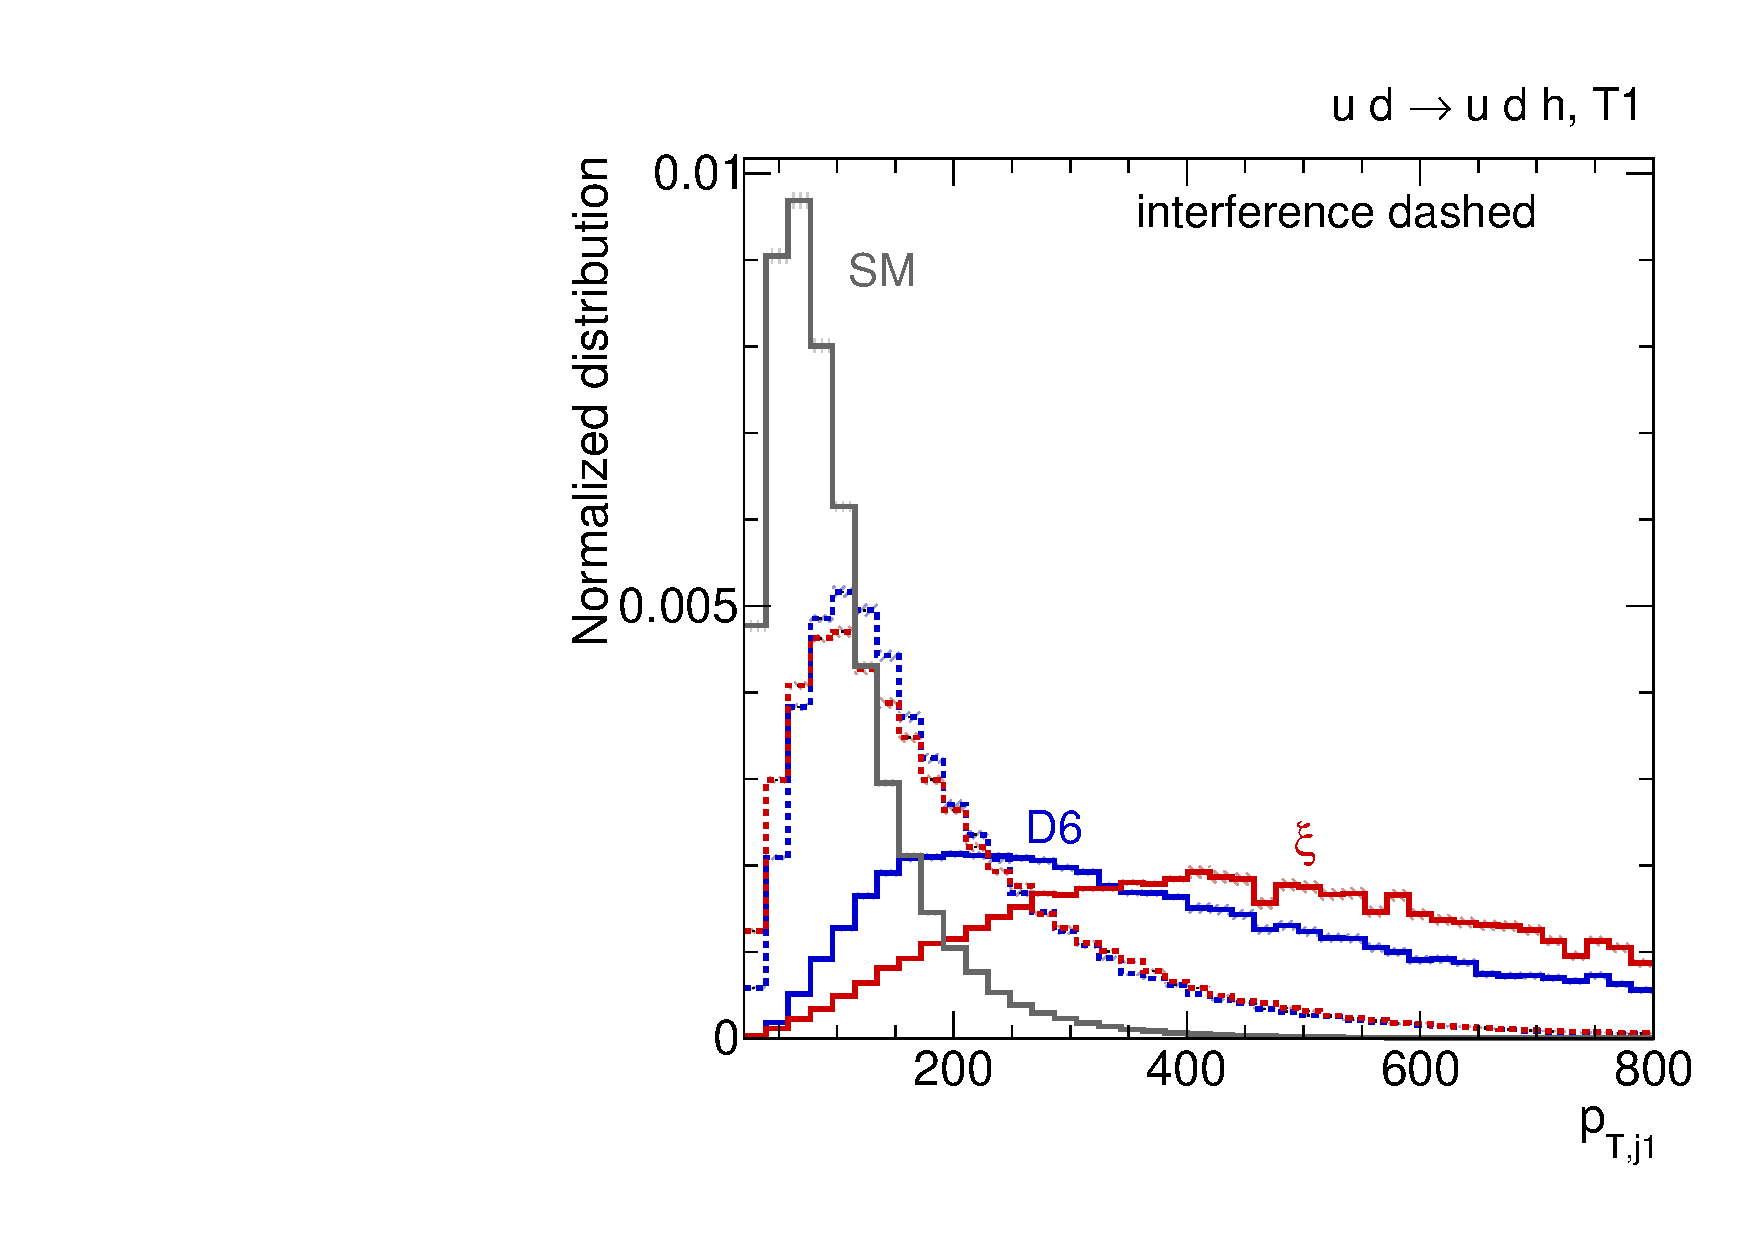
\includegraphics[width=0.49\textwidth]{fig/validity/WBF_separate_T1_j1pt.pdf}%
%   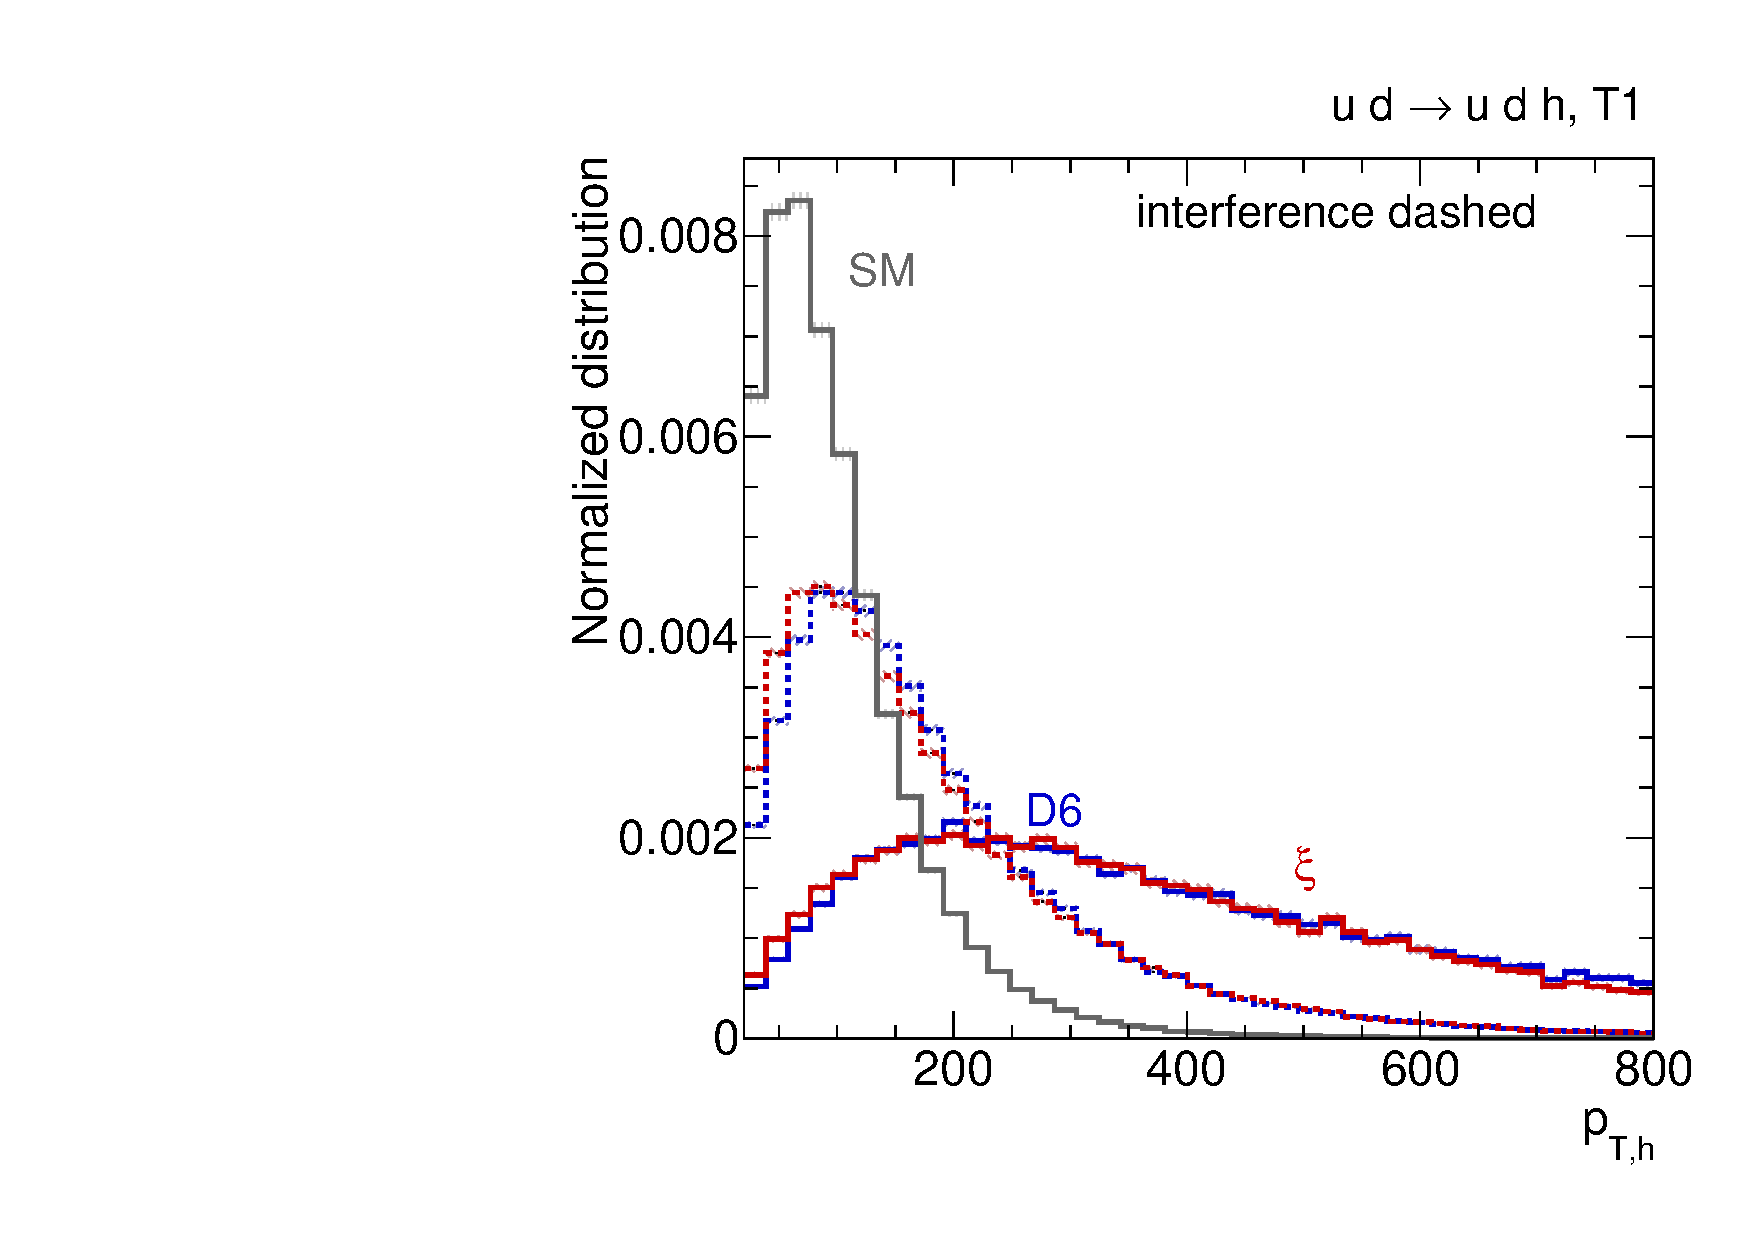
\includegraphics[width=0.49\textwidth]{fig/validity/WBF_separate_T1_Hpt.pdf}\\%
%   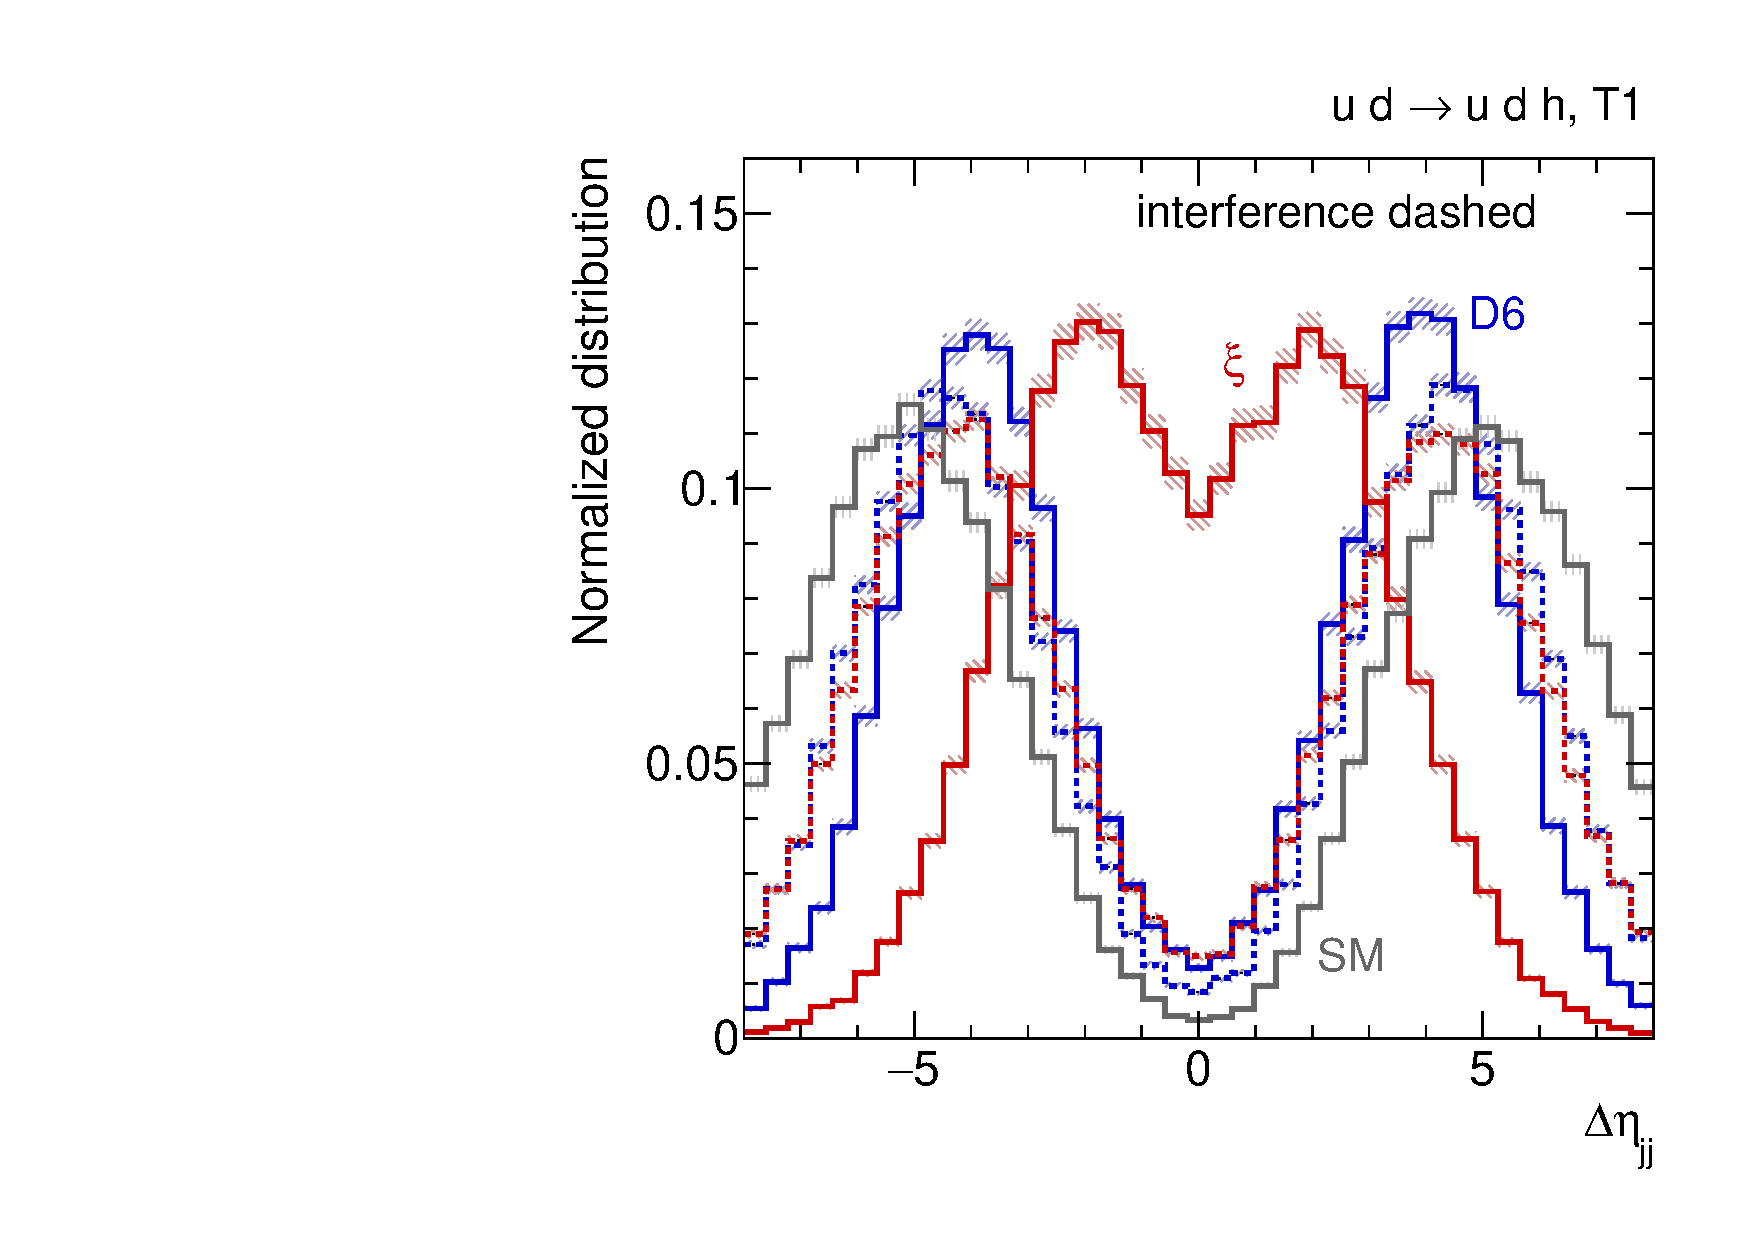
\includegraphics[width=0.49\textwidth]{fig/validity/WBF_separate_T1_deltaEtaJJ.pdf}%
%   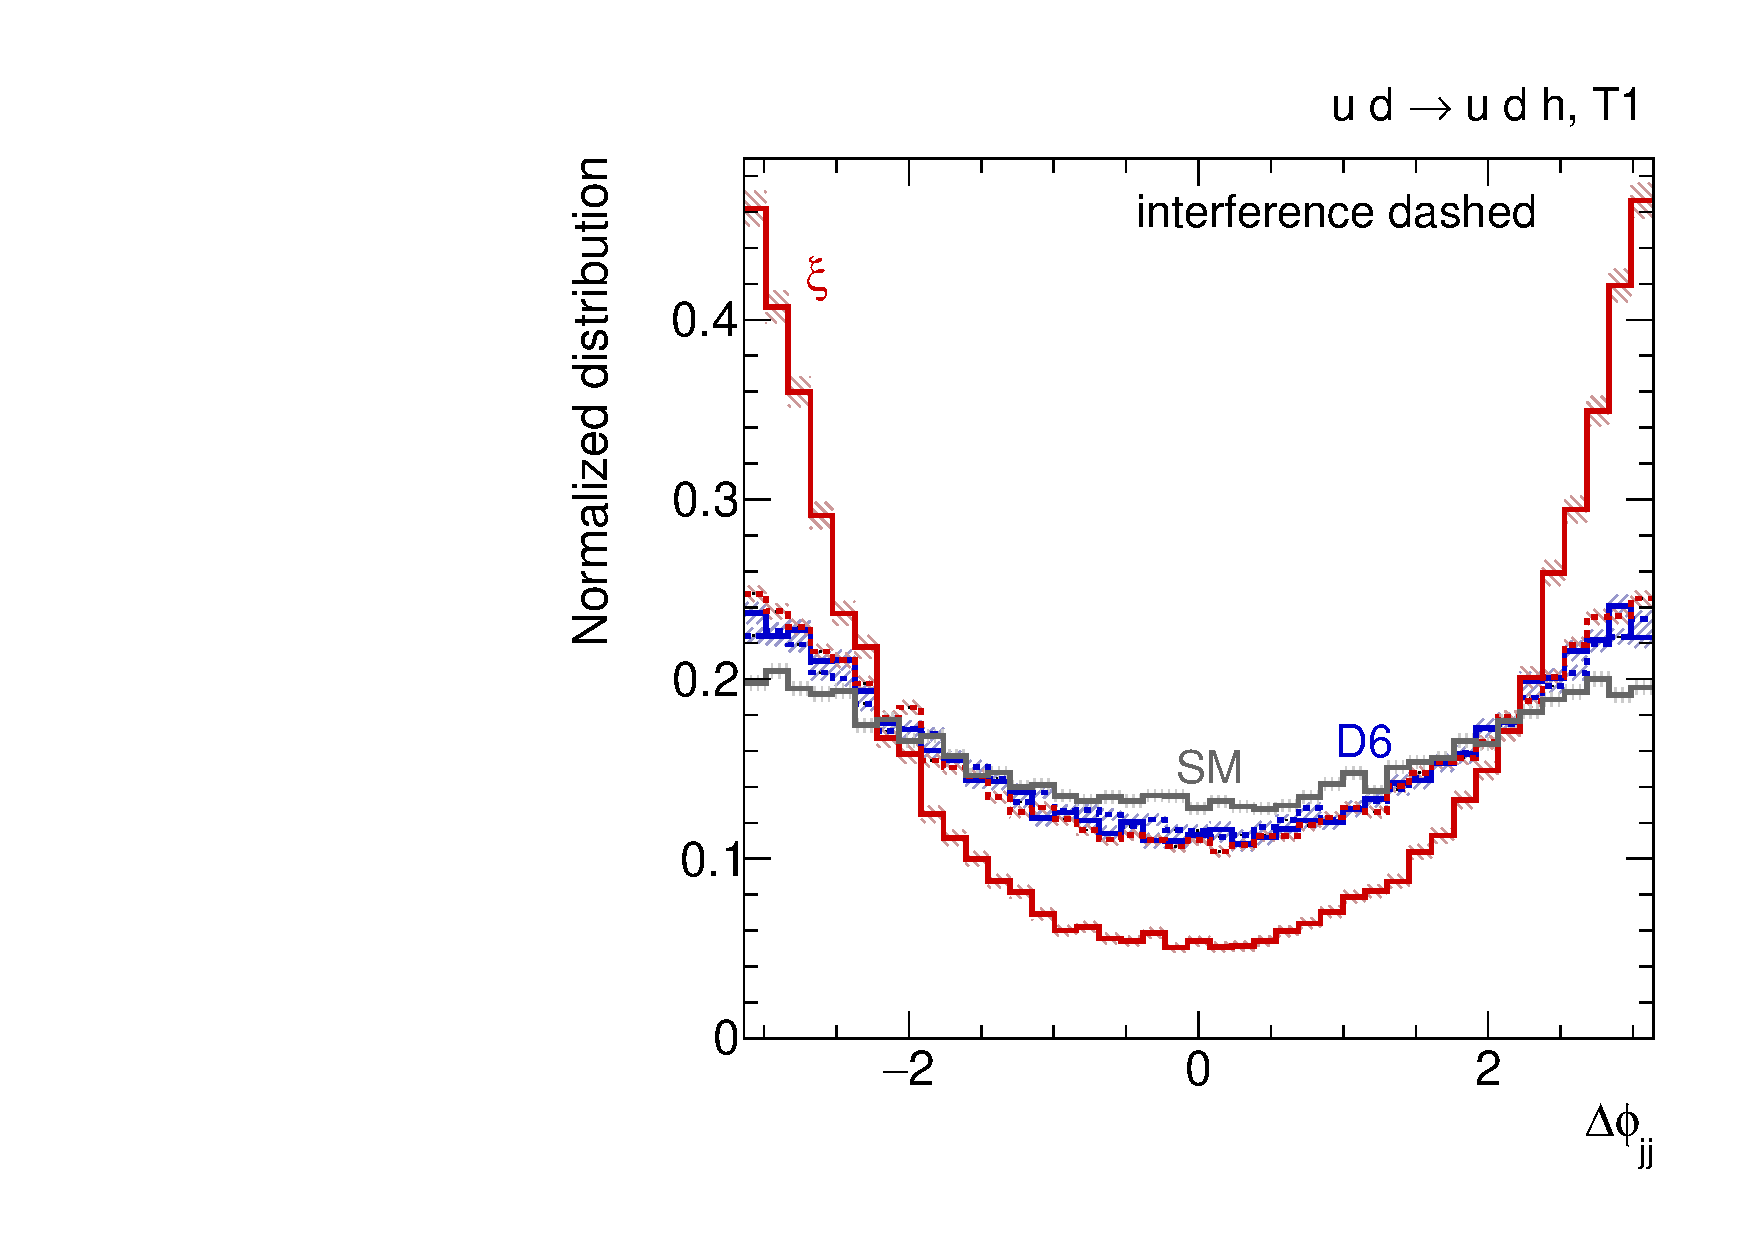
\includegraphics[width=0.49\textwidth]{fig/validity/WBF_separate_T1_deltaPhiJJ.pdf}%
%   \caption{Normalised WBF distributions of the tagging jets. We separate
%     the squared new-physics amplitudes, shown as solid lines, from the
%     interference with the SM-like diagrams (dashed).}
%   \label{fig:validity_squared_separate}
% \end{figure}

% In the first part of the paper we have shown where in phase space a
% dimension-six description of LHC observables breaks down, both for $Vh$
% production and for weak boson fusion. For $Vh$ production with its
% simple $2 \to 2$ kinematics problems are clearly linked to a possible
% $s$-channel resonance, as seen in Equation\;\eqref{eq:validity_breakdown_vh}.  For
% weak boson fusion there appears no resonance, but the result of
% Equation\;\eqref{eq:validity_breakdown_wbf} suggests that the new states in the
% $t$-channel have a similar effect.  In \autoref{fig:validity_squared_separate}
% we show different tagging jet distributions, separating the Feynman
% diagrams including the heavy $\xi$ states. In particular for the
% critical $p_{T,j_1}$ distribution, the $\Delta \eta_{jj}$
% distribution, and the $\Delta \phi_{jj}$ distribution these diagrams
% are only very poorly described by the dimension-six approach. In
% practice this is not a problem because these contributions are
% strongly suppressed by the heavy mass $m_\xi$, but it poses the
% question how we can improve the agreement. The obvious solution to
% these problems in the $s$-channel of $Vh$ production and in the
% $t$-channel of weak boson fusion is a simplified
% model~\cite{simp,simp_higgs}. A new vector field mixing with the weak
% bosons as described by the Lagrangian shown in
% Equation\;\eqref{eq:validity_lag-vectortriplet} is such a simplified model, but its
% structure is still relatively complex. Obviously, an additional heavy
% scalar with mass around $m_\xi$ and the appropriate couplings will
% improve the $2 \to 2$ kinematics for $Vh$ production. The question we
% want to study in this section is if such a scalar can also improve the
% weak boson fusion kinematics.



% %%%%%%%%%%%%%%%%%%%%%%%%%%%%%%%%%%%%%%%%%%%%%%%%%%%%%%%%%%%%
% \subsubsection*{A pseudo-scalar as a simplified vector}
% %%%%%%%%%%%%%%%%%%%%%%%%%%%%%%%%%%%%%%%%%%%%%%%%%%%%%%%%%%%%

% The simplest simplified model we can write down includes one new
% massive scalar $S$ with a Higgs portal and a Yukawa coupling. 
% However, a scalar state will not interfere with the Standard Model
% diagrams. In analogy to the CP properties of the Goldstone mode
% contributing to the massive $Z$ boson we define our simplified model
% with a pseudo-scalar state as
% %
% \begin{align}
% \mathcal{L} \supset 
%   \frac{1}{2} (\partial_\mu S)^2 
% - \frac{m_S}{2} S^2 
% + \sum_\text{fermions} g_F \; S \overline{F} \gamma_5 F 
% + g_S \; S^2 \phi^\dagger \phi \,.
%   \label{eq:validity_simplified_model}
% \end{align}

% %------------------------------------------------------------
% \begin{figure}[t]
%   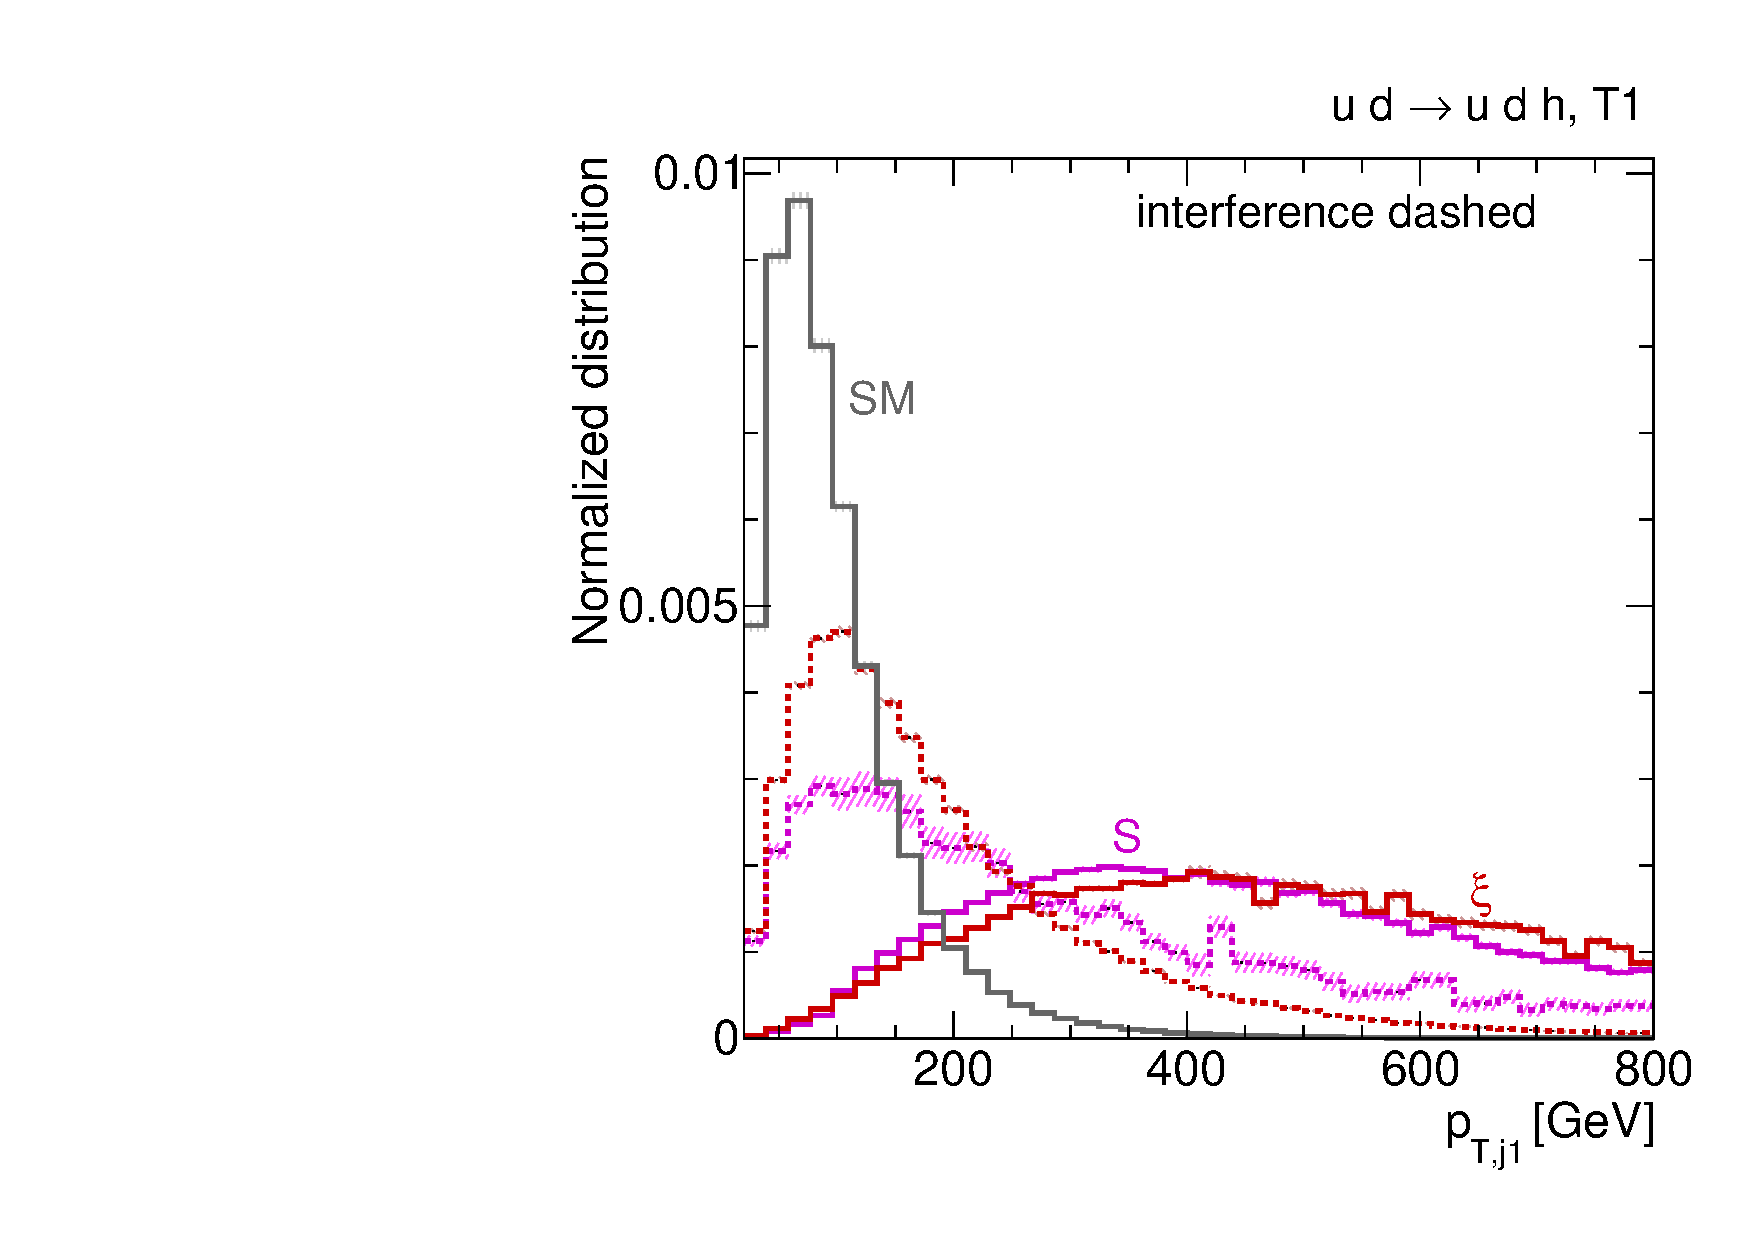
\includegraphics[width=0.43\textwidth]{fig/validity/WBF_simplified_j1pt.pdf}
%   \hspace*{0.05\textwidth}
%   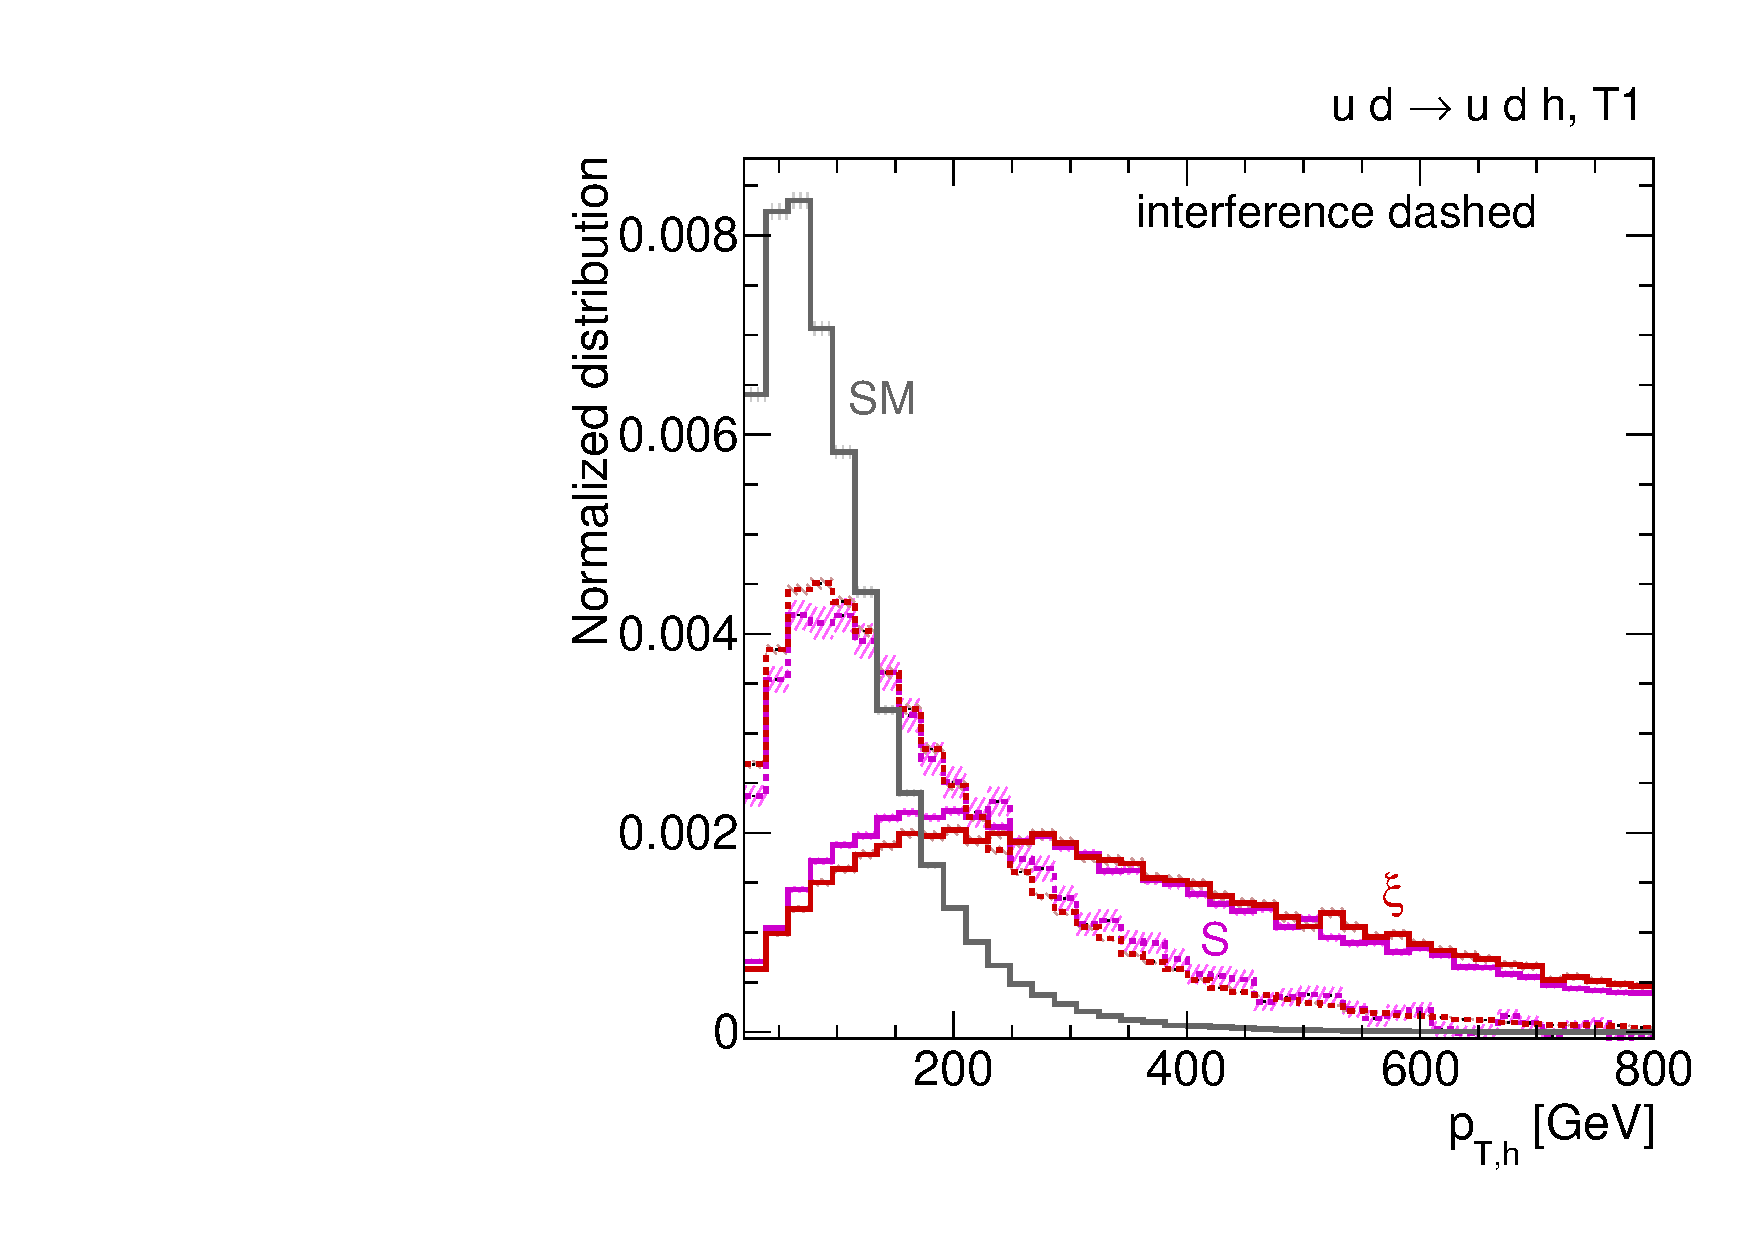
\includegraphics[width=0.43\textwidth]{fig/validity/WBF_simplified_Hpt.pdf} \\
%   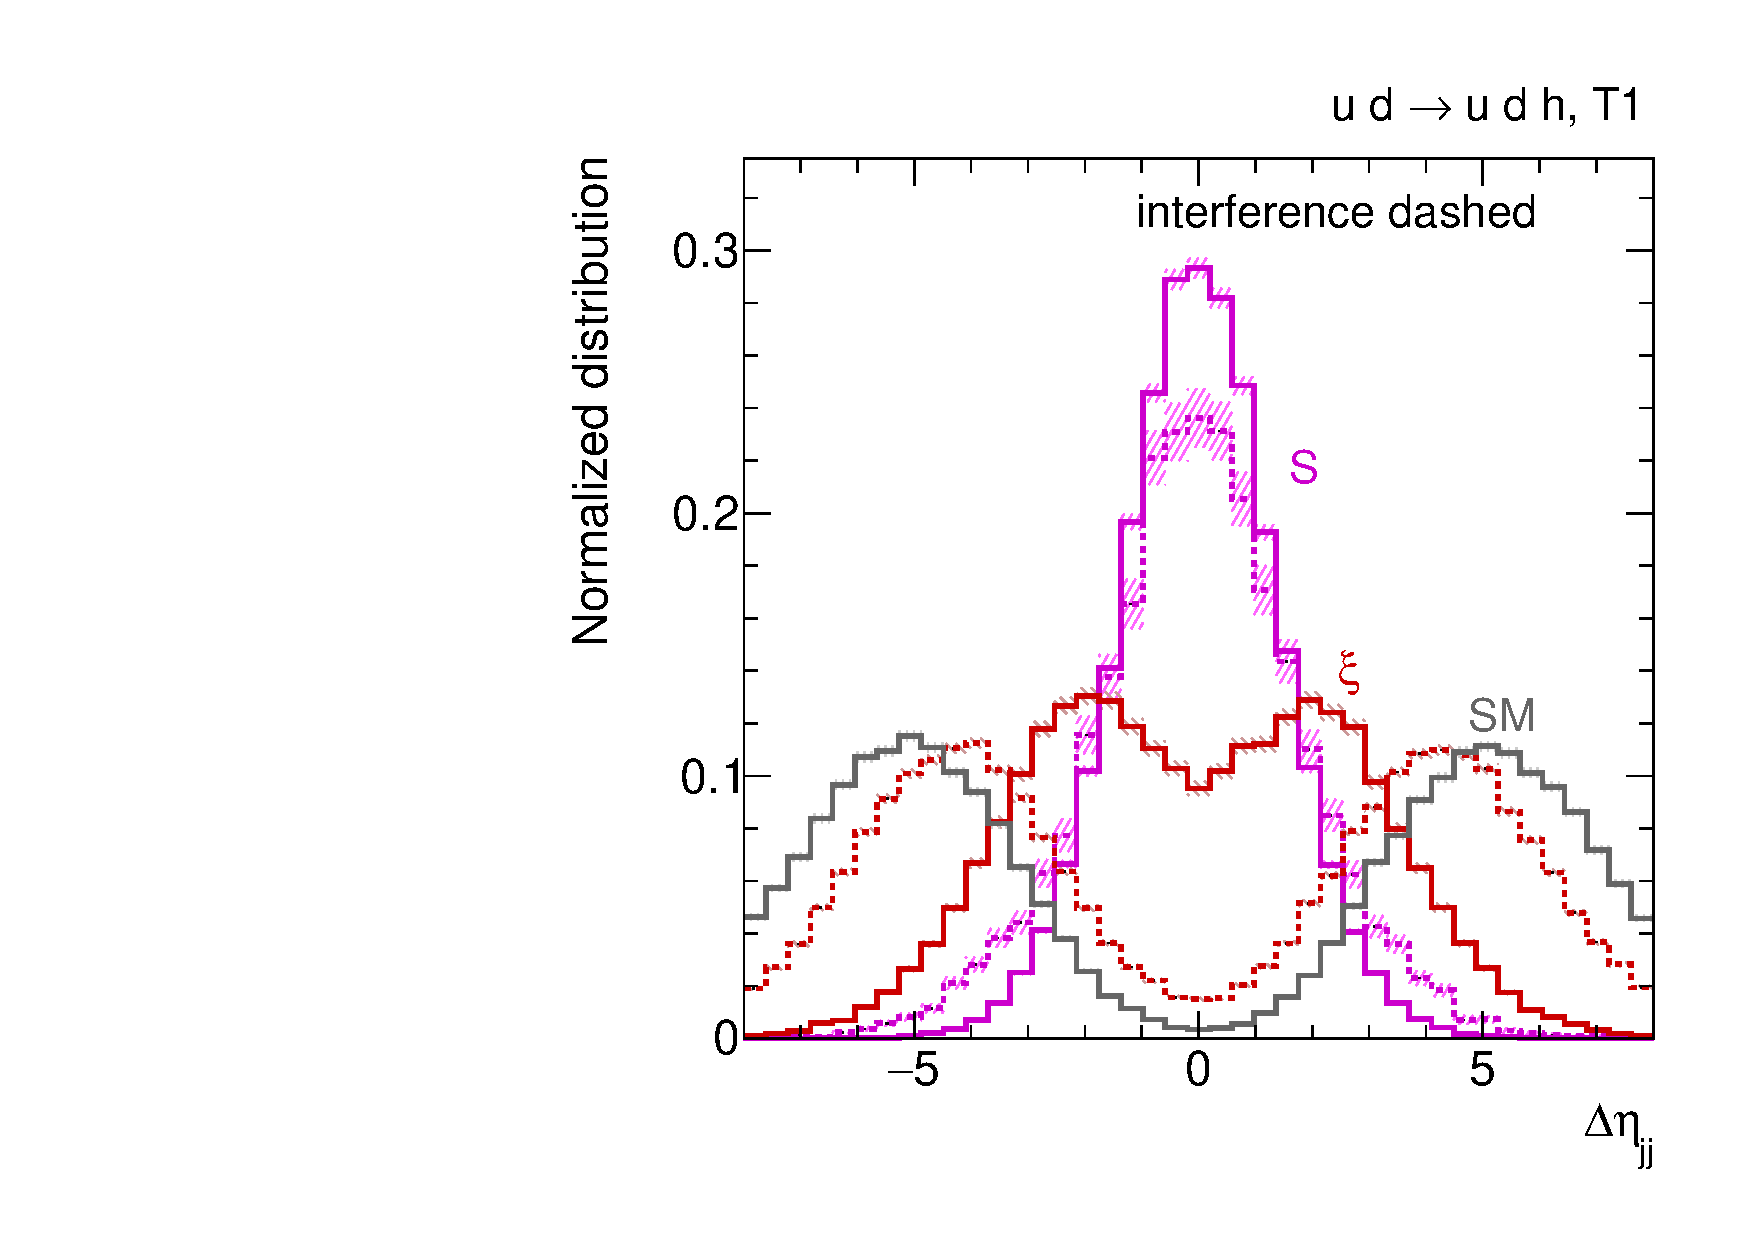
\includegraphics[width=0.43\textwidth]{fig/validity/WBF_simplified_deltaEtaJJ.pdf}
%   \hspace*{0.05\textwidth}
%   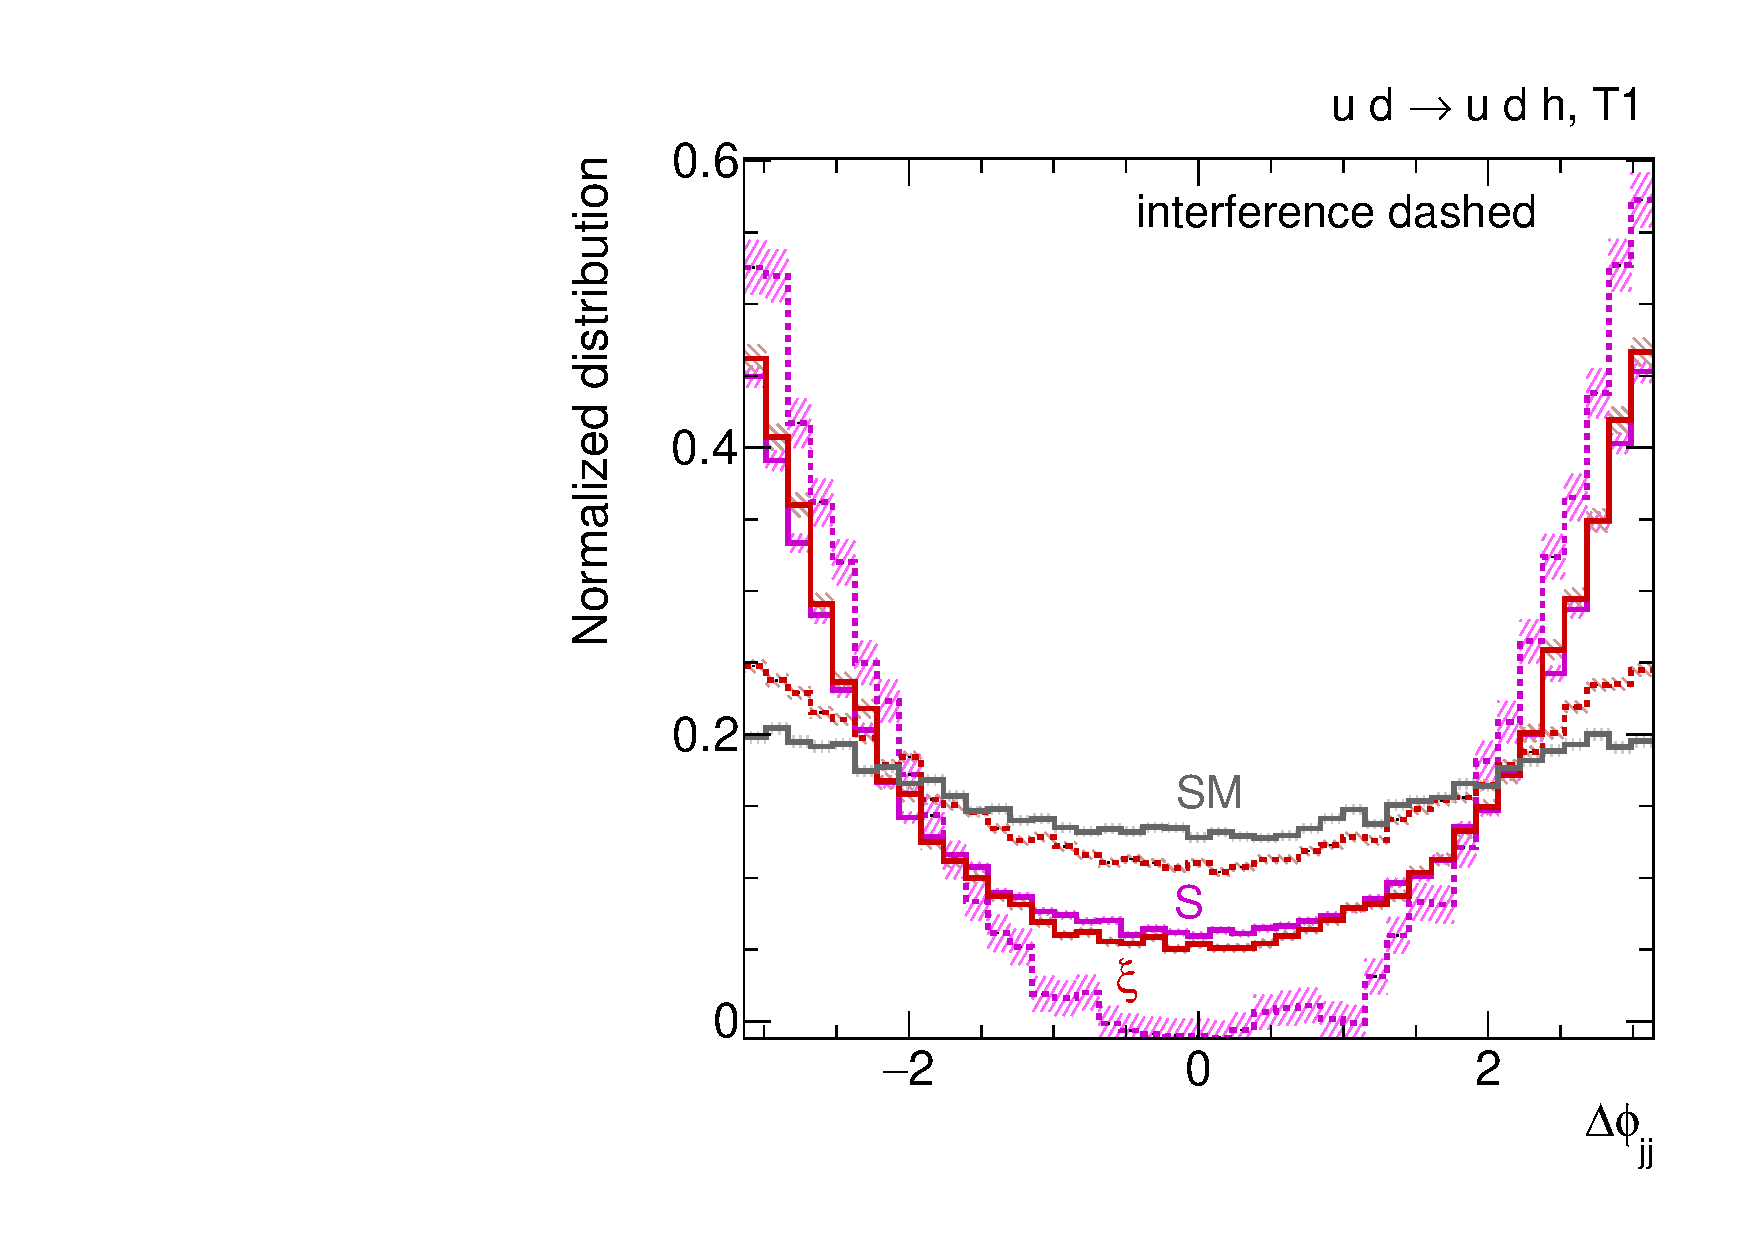
\includegraphics[width=0.43\textwidth]{fig/validity/WBF_simplified_deltaPhiJJ.pdf}
%   \caption{Normalised WBF distributions for a scalar simplified model
%     defined in Equation\;\eqref{eq:validity_simplified_model} vs the vector triplet
%     benchmark.}
%   \label{fig:validity_simplified}
% \end{figure}
% %------------------------------------------------------------

% In \autoref{fig:validity_simplified} we show the same WBF distributions as in
% \autoref{fig:validity_squared_separate}, but including the simplified scalar
% model. For the $p_{T,j}$ distribution the squared new-physics
% amplitudes in the full vector model and the simplified scalar model
% indeed agree well, improving upon the dimension-six description which
% breaks down in this distribution.  However, the interference term with
% the Standard Model, which is numerically dominant for most of the
% distribution and well described in the dimension-six model, poses a
% problem.  The $\Delta \eta_{jj}$ distributions show even poorer
% agreement: the spin-1 amplitudes of the Standard Model and the vector
% triplet have similar phase-space distributions and give two forward
% tagging jets, while the scalar mediator favours central
% jets~\cite{spins2}.  The $\Delta \phi_{jj}$ distribution, known to be
% sensitive to the tensor structure of the hard $VVh$
% interaction~\cite{delta_phi}, exposes similar differences between the
% full and simplified model.  Altogether, our simplified scalar model
% with its very different $VVh$ interaction structure does improve the
% description in the region where the dimension-six approach breaks down,
% but it fails to describe interference patterns and angular
% correlations of the tagging jets.



% %%%%%%%%%%%%%%%%%%%%%%%%%%%%%%%%%%%%%%%%%%%%%%%%%%%%%%%%%%%%
% \subsubsection*{Splitting functions and equivalence theorem}
% %%%%%%%%%%%%%%%%%%%%%%%%%%%%%%%%%%%%%%%%%%%%%%%%%%%%%%%%%%%%

% We can understand this very different behaviour of the scalar
% $t$-channel mediator as compared to the vector from the splitting
% kernels in the collinear limit.  The matrix element squared for the
% weak boson fusion process mediated by pseudo-scalars $S$ has the form
% %
% \begin{align}
%  | \mathcal{M}(qq \to q'q'h) |^2 \propto 
%   \frac{g_F^4 \;  t_1 t_2}{(t_1 - m_S^2)^2 \; (t_2 - m_S^2)^2} 
% \stackrel{m_S \to 0}{\longrightarrow} \frac{\text{const}}{t_1 t_2} \; ,
% \end{align}
% %
% where $t_1$ and $t_2$ denote the respective momentum flow through each
% scalar propagator. For $m_S \to 0$ the Jacobians from the phase-space
% integration cancel a possible collinear divergence, while for a light
% vector boson a soft and a collinear divergence remains. Unlike in the
% usual WBF process, the tagging jets in our simplified scalar model
% will not be forward.  The reason for this difference in the
% infrared is the (pseudo-)scalar coupling to quarks: since the scalar
% carries no Lorentz index, a $q \to q S$ splitting will be expressed in
% terms of the momentum combinations $(p_q p_q')$, $p_q^2 = m_q^2$, and
% $p_q'^2 = m_q^2$. In the limit of massless quarks only the first term
% remains as $t = 2 (p_q p_q')$.  This factor in the numerator cancels
% the apparent divergence of the $t$-channel propagator.

% Adding higher-dimensional couplings of the (pseudo-)scalar to
% fermions, such as
% %
% \begin{align}
%   \mathcal{L} \supset 
% \sum_\text{fermions} \Biggl[  
%   g_{F,2} S \overline{F} F 
% + g_{F,3} (\partial_\mu S) \overline{F} \gamma^\mu F
% + g_{F,4} S (\partial_\mu S) \overline{F} \gamma^\mu \gamma_5 F 
% + g_{F,5} S (\partial_\mu \partial_\nu S) \overline{F} [\gamma^\mu,\gamma^\nu] F
% \Biggr] \; ,
% \label{eq:validity_simplified_model_extended}
% \end{align}
% %
% does not change this result qualitatively. After partial integration
% and using the Dirac equation for the on-shell quarks the coupling
% $g_{F,3}$ is equivalent to the simple scalar coupling, $g_{F,2} = m_q^2
% g_{F,3}$. In the limit of massless quarks, only two of the new
% structures listed in Equation\;\eqref{eq:validity_simplified_model_extended}
% contribute at all: $g_{F,2}$ gives exactly the same result as $g_F$,
% while $g_{F,5}$ leads to even higher powers of $t$ in the numerator,
% %
% \begin{align}
%   | \mathcal{M}(qq \to q'q'h) |^2 \propto 
%   \frac{g_{F,5}^4 \; t_1^3 t_2^3}{(t_1 - m_s^2)^2 \; (t_2 - m_s^2)^2} \; . 
% \end{align}
% %
% No matter how we couple the (pseudo-)scalar of the simplified model to
% the external quarks, it never reproduces the collinear splitting
% kernel of a vector boson.

% To be a little more precise, we can write out the spin-averaged matrix
% element squared for the $q \to q' S$ splitting in terms of the energy
% of the initial quark $E$, the longitudinal momentum fraction $x$, and
% the transverse momentum $p_T$, both carried by $S$,
% %
% \begin{align}
%  | \mathcal{M}(q \to q'S) |^2 &= - 2 g_F^2 x m_q^2
%                      + 2 g_F^2 E^2 (1-x)
%                      \Biggl[ \sqrt{1 + \frac {p_T^2} {E^2 (1-x)^2} + \frac {m_q^2 (1 - (1-x)^2)} {E^2 (1-x)^2} } - 1 \Biggr] \notag \\
%                    &= g_F^2 \, \frac {x^2 \, m_q^2} {1-x} 
%                      + g_F^2 \,  \frac {p_T^2} {1-x} 
%                      + \ord { \frac{m_q^2 p_T^2}{E^2}, \frac{m_q^4}{E^2}, \frac{p_T^4}{E^2} } \;.
% \label{eq:validity_splitting_s}
% \end{align}
% %
% From Equation\;\eqref{eq:validity_splitting_s} one can derive an effective Higgs
% approximation or \emph{effective scalar
%   approximation}~\cite{effective_scalar}: in the collinear and
% high-energy limit, a process $q X \to q' Y$ mediated by a
% (pseudo-)scalar $S$ is described by
% %
% \begin{align}
%   \sigma (qX \to q'Y) = \int \mathrm{d}x \, \mathrm{d} p_T \, F_S(x,p_T)
%   \, \sigma (SX \to Y)
% \label{eq:validity_def_splitting}
% \end{align}
% %
% with the splitting function
% %
% \begin{align}
%   F_S(x,p_T) &= \frac {g_F^2} {16 \pi^2} \, 
%                \frac {x \, p_T^3} {\left( m_S^2 (1-x) + p_T^2 \right)^2} \,.
% \label{eq:validity_kernel_s}
% \end{align}
% %
% Unlike for vector emission, there is no soft divergence for $x \to 0$.
% The $p_T$ dependence is the same as for transverse vector
% bosons~\cite{effective_w,polarized_ww}, as we discuss in some detail in the
% appendix. 

% It might seem surprising that our pseudo-scalar is emitted with a
% fundamentally different phase-space dependence than longitudinal $W$
% and $Z$ bosons, in apparent contradiction of the Goldstone boson
% equivalence theorem.  However, the latter only makes a statement about
% the leading term in an expansion in $m_W / E$, where 
% $\varepsilon^\mu_L \sim p^\mu / m_W$. At this order the squared matrix
% element for the splitting $q \to q' W_L$ agrees with the pseudo-scalar
% result, but is suppressed by a factor of $m_q^2 / E^2$. Higher orders
% in the $m_W/E$ expansion, outside the validity range of the
% equivalence theorem, are not suppressed by quark masses.  The
% equivalence theorem is therefore of very limited use in describing the
% $W$ or $Z$ couplings to quarks except the top.

% %%%%%%%%%%%%%%%%%%%%%%%%%%%%%%%%%%%%%%%%

% In Sec.~\ref{sec:validity_simplified} we have introduced a pseudo-scalar in the
% $t$-channel of weak boson fusion to describe some of the features
% which we find in the full vector triplet model and which our
% dimension-six description does not describe well. In this appendix we
% collect some of the main formulas and compare the kinematics of
% fermions radiating scalars, transverse, or longitudinal gauge
% bosons. Our formalism follows the effective
% $W$ approximation~\cite{effective_w} as well as the effective Higgs
% approximation~\cite{effective_scalar} and allows us to analytically
% describe the soft and collinear behaviour. If we do not need to
% describe interference terms with SM gauge bosons we can start with a
% CP-even scalar splitting $q \to qS$, in terms of the energy of the
% initial quark $E$, the longitudinal momentum fraction $x$, carried by $S$, and the
% scalar's transverse momentum $p_T$:
% %
% \begin{align}
%  | \mathcal{M}(q \to q'S)  |^2 &= 2 g_F^2 (2-x) m_q^2
%                      + 2 g_F^2 E^2 (1-x)
%                      \Biggl[ \sqrt{1 + \frac {p_T^2} {E^2 (1-x)^2} + \frac {m_q^2 (1 - (1-x)^2)} {E^2 (1-x)^2} } 
%                        - 1 \Biggr] \notag \\
%                    &= g_F^2 \left( 4  + \frac {x^2} {1-x} \right) m_q^2
%                      + g_F^2 \, \frac {p_T^2} {1-x} 
%                      + \ord {\frac{m_q^2 p_T^2}{E^2}, \frac{m_q^4}{E^2}, \frac{p_T^4}{E^2} } \; .
% \end{align}
% %
% The main feature of this splitting is that the infrared behaviour is
% different for the term proportional to the quark mass and for the
% surviving term in the realistic limit $m_q \to 0$: in the absence of a
% fermion mass the collinear divergence from a $t$-channel propagator is
% cancelled by the coupling structure. If the term proportional to $m_q$
% dominates there will be the usual collinear divergence once we include
% a scalar propagator. For a pseudo-scalar the structure shown in
% Equation\;\eqref{eq:validity_splitting_s} is very similar,
% %
% \begin{align}
%  |\mathcal{M}(q \to q'S)  |^2 &= - 2 g_F^2 x m_q^2
%                      + 2 g_F^2 E^2 (1-x)
%                      \Biggl[ \sqrt{1 + \frac {p_T^2} {E^2 (1-x)^2} + \frac {m_q^2 (1 - (1-x)^2)} {E^2 (1-x)^2} } 
%                                 - 1 \Biggr] \notag \\
%                    &= g_F^2 \, \frac {x^2 \, m_q^2} {1-x} 
%                      + g_F^2 \,  \frac {p_T^2} {1-x} 
%                      + \ord {\frac{m_q^2 p_T^2}{E^2}, \frac{m_q^4}{E^2}, \frac{p_T^4}{E^2} } \;.
% \end{align}

% In the limit $m_q \to 0$ we can compute universal splitting kernels
% including only the leading term in $p_T$, as defined in
% Equation\;\eqref{eq:validity_def_splitting}.  Obviously, the scalar and pseudoscalar
% case given in Equation\;\eqref{eq:validity_kernel_s} are identical, and we can compare
% them with the splitting kernels for longitudinal or transverse
% $W$ bosons~\cite{effective_w},
% %
% \begin{align}
%   F_S(x,p_T) &= \frac {g_F^2} {16 \pi^2} \, x \,
%                \frac {p_T^3} {\left( m_S^2 (1-x) + p_T^2 \right)^2} \,,\notag \\
%   F_T(x,p_T) &= \frac {g^2} {16 \pi^2} \, \frac {1+(1-x)^2} x \, \frac {p_T^3} {\left( m_W^2 (1-x) + p_T^2 \right)^2} \,, \notag \\
%   F_L(x,p_T) &= \frac {g^2} {16 \pi^2} \, \frac {(1-x)^2} x \, \frac {2 m_W^2 \, p_T} {\left( m_W^2 (1-x) + p_T^2 \right)^2} \,.
%   \label{eq:validity_splittings}
% \end{align}

% In \autoref{fig:validity_effective_scalar} we show how these different
% splittings translate into WBF distributions and compare full simulations
% in \toolfont{MadGraph} to the predictions of Equation\;\eqref{eq:validity_splittings}.
% A heavy Higgs, $m_h = 1$~TeV, is needed to guarantee a large energy scale
% $E \sim m_h \gg p_T \sim m_W, m_S$. In this case we find that the
% effective scalar approximation quite accurately describes the transverse
% momentum distribution of the tagging jets. For $m_h = 125$~GeV the
% assumption of on-shell $W$ bosons or scalars breaks down and the
% effective descriptions lose their validity.

% \begin{figure}
%   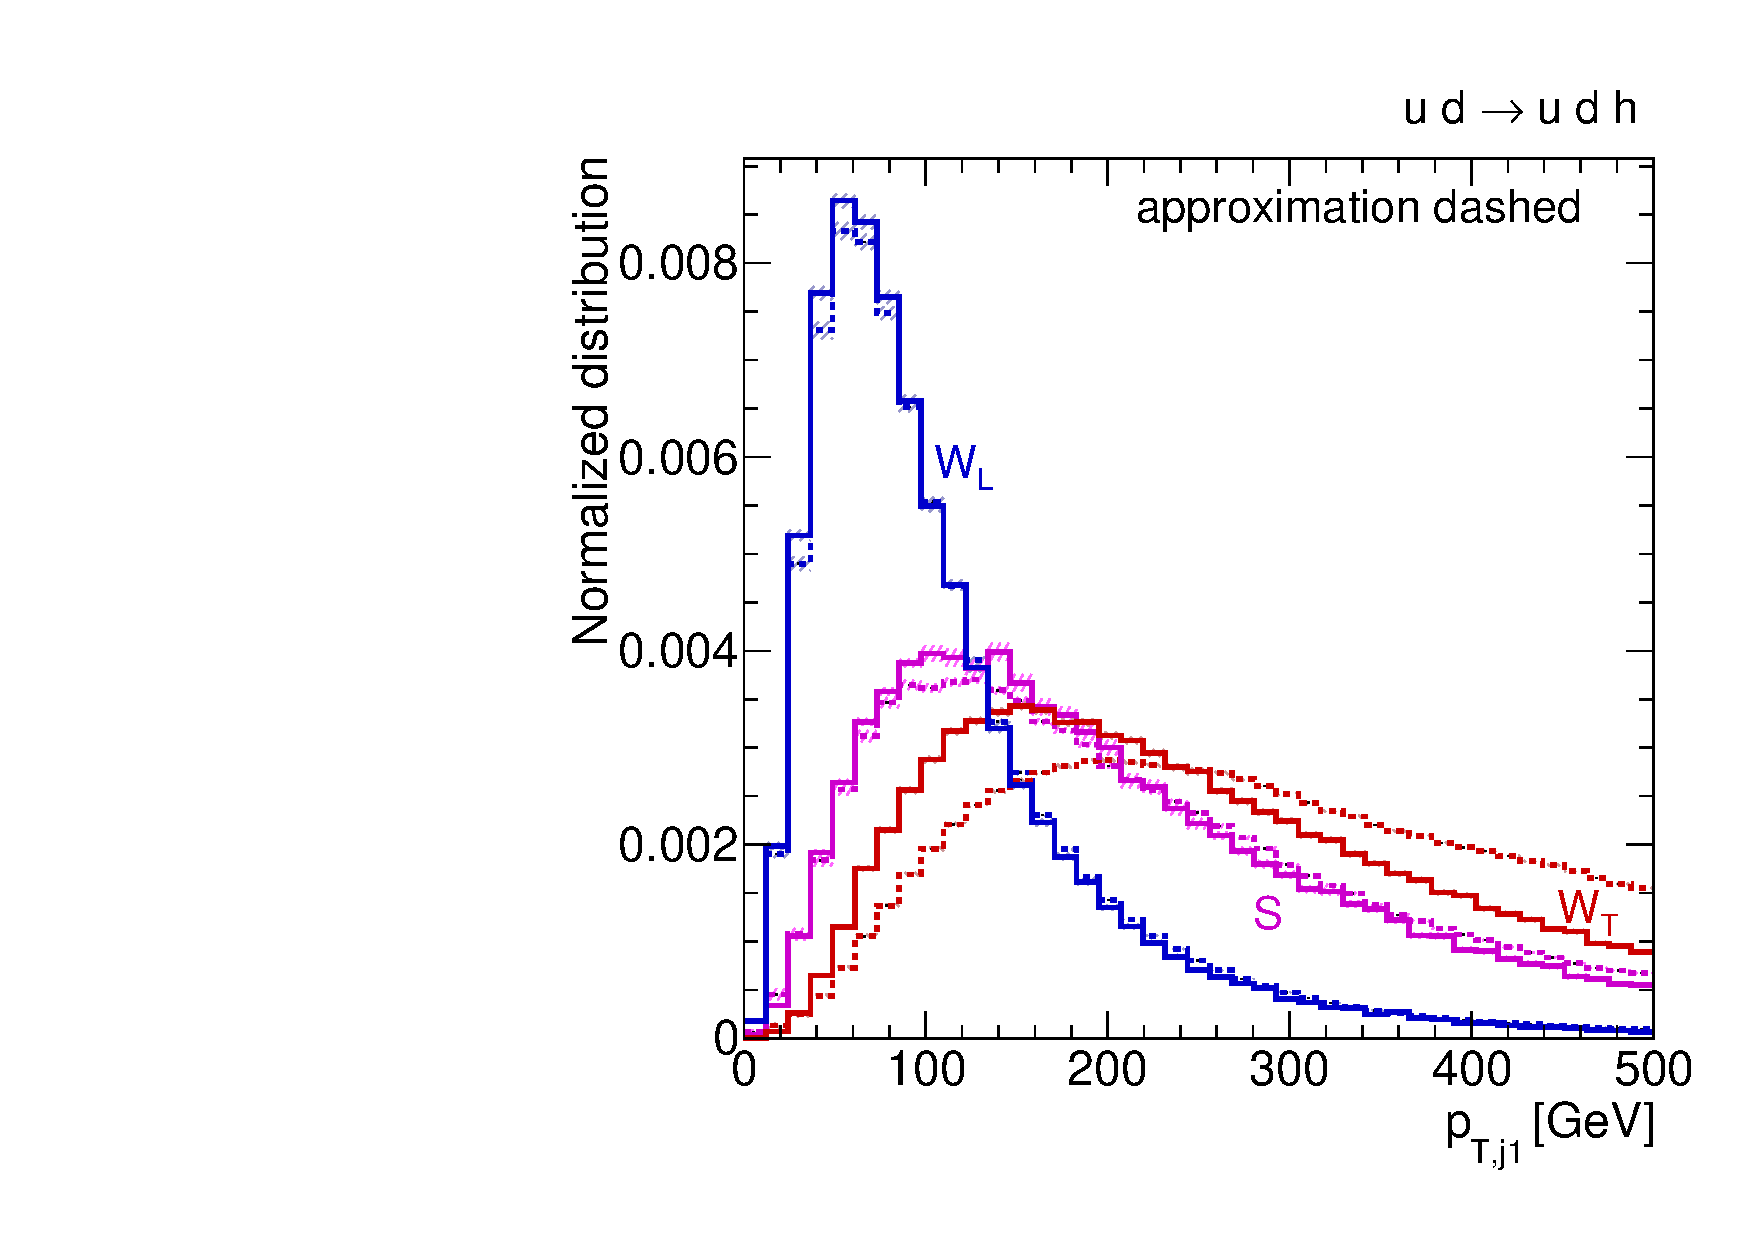
\includegraphics[width=0.43\textwidth]{fig/validity/WBF_ESA.pdf}
%   \caption{Normalised WBF distributions of the tagging jets in the SM with
%   a heavy Higgs, $m_h = 1$~TeV. Scalar mediators are compared to
%   longitudinal and transverse $W$ bosons following
%   Reference~\cite{polarized_ww}.
%   The dotted lines give the corresponding predictions of the effective
%   $W$ and scalar approximations, \autoref{eq:validity_splittings}.}
%   \label{fig:validity_effective_scalar}
% \end{figure}





%%%%%%%%%%%%%%%%%%%%%%%%%%%%%%%%%%%%%%%%%%%%%%%%%%%%%%%%%%%%
\section{Fisher information derivations}
\label{sec:appendix_information}
%%%%%%%%%%%%%%%%%%%%%%%%%%%%%%%%%%%%%%%%%%%%%%%%%%%%%%%%%%%%